\section{Bi-orthogonal Bases}\label{sec: bi-orth}
In this section, we analyze bi-orthogonal bases in the following form of MRA,
\begin{align}\label{eq: bi-orth MRA}
\{\phi_{L,\V{k}},\widetilde{\phi}_{L,\V{k}}, \psi_{l,\V{k}'}^j,\widetilde{\psi}_{l,\V{k}'}^j,\, 1\leq l\leq L,\,\V{k}\in\mathbb{Z}^2,\, \V{k}'\in\mathbf{Q}\mathbb{Z}^2,\,1\leq j\leq J \},
\end{align}
where $\phi$ and $\psi^j$ satisfy \eqref{eq: m0} and \eqref{eq: mj}, as well as $\widetilde{\phi}$ and $\widetilde{\psi^j}$, respectively,
\begin{align}\label{eq: mj_dual}
\widehat{\widetilde{\phi}}(\V{D}^T\V{\omega}) = \widetilde{m_0}(\V{\omega})\widehat{\widetilde{\phi}}(\V{\omega}),\quad \widehat{\widetilde{\psi^j}}(\V{D}^T\V{\omega}) = \widetilde{m_j}(\V{\omega})\widehat{\widetilde{\phi}}(\V{\omega}).
\end{align}
For such bi-orthogonal bases, we have the similar identity summation and shift cancellation conditions to those in Theorem \ref{thm: conds}.
\begin{thm}\label{thm: bi-orth conds}
The perfect reconstruction iff the following two conditions hold
\begin{align}\label{eq: id-sum 2}
m_0(\boldsymbol{\omega})\sbarm{0} + \sum_{j = 1}^6 m_j(\boldsymbol{\omega})\sbarm{j} = 1
\end{align}
\begin{equation}\label{eq: shift-cancel 2}
\begin{cases}
\sum_{j = 0}^6m_j(\boldsymbol{\omega})\overlinespace{\widetilde{m_j}}(\boldsymbol{\omega} + \boldsymbol{\pi}) = 0, & \boldsymbol{\pi}\in \Gamma_0\setminus\{\boldsymbol{0}\}\\[.5em]
\sum_{j=1}^6m_j(\boldsymbol{\omega})\overlinespace{\widetilde{m_j}}(\boldsymbol{\omega}+\boldsymbol{\pi}) = 0, & \boldsymbol{\pi}\in\Gamma_1\setminus\Gamma_0
\end{cases}
\end{equation}
\end{thm}
\vspace{1em}
%where $\M\in\mathbb{C}^{8\times 7}$ and $\mathbf{m}_0\in\mathbb{C}^7$.
We also have the following analogue of Theorem \ref{thm: basis cond}.
\begin{thm}\label{thm: basis cond 2}
Assume that $m_0, \widetilde{m_0}$ are trigonometric polynomials with $m_0(\V{0})=\widetilde{m_0}(\V{0}) = 1$, which generate $\phi,\widetilde{\phi}$ respectively.\\
If $\phi(\cdot - \boldsymbol{k}),\widetilde{\phi}(\cdot - \boldsymbol{k}),\,\boldsymbol{k}\in\mathbb{Z}^2$ are bi-orthogonal, then $\exists K$ containing a neighborhood of 0, s.t. $\forall\boldsymbol{\omega}\in S_0,\,\boldsymbol{\omega}+2\pi\mathbf{n}\in K$ for some $\mathbf{n}\in\mathbb{Z}^2, $ and $\inf_{k>0,\,\boldsymbol{\omega}\in K}|m_0(\mathbf{D_2}^{-k}\boldsymbol{\omega})| >0$, $\inf_{k>0,\,\boldsymbol{\omega}\in K}|\widetilde{m_0}(\mathbf{D_2}^{-k}\boldsymbol{\omega})| >0$. 
 Furthermore, if  $\sum_{\boldsymbol{\V{\pi}}\in \Gamma_0} m_0(\boldsymbol{\omega}+\boldsymbol{\pi})\sbarmp{0}{} = 1,$ then the inverse is true.
\end{thm}
By Theorem \ref{thm: basis cond 2}, $m_0$ and $\widetilde{m_0}$ need to satisfy the following identity constraint for the MRA \eqref{eq: bi-orth MRA} to be bi-orthogonal,
\begin{align}\label{eq: identity-cond}
m_0\sbarm{0} + m_0\sbarmp{0}{2} + m_0\sbarmp{0}{4} + m_0\sbarmp{0}{6} = 1.
\end{align}
In addition, the identity summation and shift cancellation conditions \eqref{eq: id-sum 2} and \eqref{eq: shift-cancel 2} from Theorem \ref{thm: bi-orth conds}
 can be combined into a linear system with respect to $m_j$ as follows,
\begin{align}\label{eq: LS-new}
%\overline{\M}(\V{\omega})\mathbf{m}_0(\V{\omega})=
\begin{bmatrix}
    \,\sbarm{0} & \sbarm{1} & \hdots & \sbarm{6}\;  \\
    \;0 & \sbarmp{1}{1}  & \hdots  & \sbarmp{6}{1}\; \\
    \,\sbarmp{0}{2} & \sbarmp{1}{2} & \hdots & \sbarmp{6}{2}\;\\
    \;\vdots & \vdots & \vdots & \vdots \; \\
    \;0 & \sbarmp{1}{7} & \hdots & \sbarmp{6}{7}\;
\end{bmatrix}
\begin{bmatrix}
\;\mo{0}\; \\
\;\mo{1}\; \\
\;\mo{2}\; \\
\; \vdots\; \\
\;\mo{6}\; 
\end{bmatrix} 
=
\begin{bmatrix}
1\\
0\\
0\\
\vdots \\
0
\end{bmatrix}
\end{align}
In sum, the construction of a bi-orthogonal basis \eqref{eq: bi-orth MRA} is equivalent to find feasible solutions of \eqref{eq: LS-new} with constraint \eqref{eq: identity-cond}\footnote{It can be shown that as long as \eqref{eq: LS-new} has a unique solution for $m_j$ given fixed $\widetilde{m_j}, \, j = 0,\cdots,6,$ \eqref{eq: identity-cond} always holds. See Section \ref{subsec: adapt-cohen}.}. To solve this, we use the same approach as in \cite{cohen1993compactly}, which constructs compactly supported symmetric bi-orthogonal filters on a hexagon lattice. We next review the main scheme in \cite{cohen1993compactly} and adapt it to our setup of bi-orthogonal bases on the dyadic quincunx lattice.

\subsection{Summary of Cohen et al's construction}\label{subsec: cohen-summary}
We summerize the main setup and the approach in \cite{cohen1993compactly}. Consider a bi-orthogonal scheme consists of three high-pass filters $m_1,m_2$ and $m_3$ and a low-pass filter $m_0$ together with their bi-orthogonal duals $\widetilde{m_j}$, s.t.
$m_0$ and $\widetilde{m_0}$ are $\frac{2\pi}{3}$-rotation invariant and $m_1,\, m_2,\, m_3$ and their duals are $\frac{2\pi}{3}$-rotation co-variant on a hexagon lattice.

This bi-orthogonal scheme satisfies the following linear system (
Lemma 2.2.2 in \cite{cohen1993compactly} )
\begin{align}\label{eq: LS}
\begin{bmatrix}
    \, \sbarm{0} &  \sbarm{1} &  \sbarm{2} & \sbarm{3}\; \\
    \;\sbarmn{0}{1} & \sbarmn{1}{1}  & \sbarmn{2}{1}  & \sbarmn{3}{1}\; \\
    \;\sbarmn{0}{2} & \sbarmn{1}{2}  & \sbarmn{2}{2}  & \sbarmn{3}{2}\; \\
    \;\sbarmn{0}{3} & \sbarmn{1}{3} & \sbarmn{2}{3} & \sbarmn{3}{3}\;
\end{bmatrix}
\begin{bmatrix}
\;\mo{0}\; \\
\;\mo{1}\; \\
\;\mo{2}\; \\
\;\mo{3}\; 
\end{bmatrix} 
=
\begin{bmatrix}
1\\
0\\
0\\
0
\end{bmatrix}
\end{align}
 where $\V{\nu}_i = \V{\pi}_{2i},\, i = 1,2,3.$ %$\V{\nu}_1 = (\pi,0),\V{\nu}_2 = (0,\pi),\V{\nu}_3=(\pi,\pi)$.
 Let $\widetilde{\mathbf{M}}(\V{\omega})\in\mathbb{C}^{4\times 4}$ be the matrix with entries $\sbarmn{j}{i}$ and $\mathbf{m}(\V{\omega})\in\mathbb{C}^4$ be the vector consisting of entries $m_j(\V{\omega})$ in \eqref{eq: LS}, then \eqref{eq: LS} can be written as \[\widetilde{\mathbf{M}}(\V{\omega})\, \mathbf{m} (\V{\omega})= [1,0,0,0]^\top.\]
Begin with a pre-designed $\m{1}$ with desired propery, $\m{2}$ and $\m{3}$ are determined by symmetry. Lemma 2.2.2 in \cite{cohen1993compactly} then leads to
\begin{align}\label{eq: m0-sol}
m_0(\V{\omega}) &= D^{-1}%\propto 
\left|
\begin{matrix}
    \; \sbarmn{1}{1}  & \sbarmn{2}{1}  & \sbarmn{3}{1}\; \\
    \; \sbarmn{1}{2}  & \sbarmn{2}{2}  & \sbarmn{3}{2}\; \\
    \; \sbarmn{1}{3} & \sbarmn{2}{3} & \sbarmn{3}{3}\;
\end{matrix}
\right| \notag\\
&= D^{-1}\widetilde{\mathbf{M}}_{0,0}(\V{\omega}),
\end{align}
where $\widetilde{\mathbf{M}}_{0,0}(\V{\omega})$ is the minor of $\widetilde{\mathbf{M}}(\V{\omega})$ with respect to $\sbarm{0}$ and $ D \equiv \det(\widetilde{\mathbf{M}}(\V{\omega}))\in \mathbb{C}^* = \mathbb{C}\setminus\{0\}$ does not depend on $\V{\omega}$ in \cite{cohen1993compactly}, due to symmetry.
%{\it Remark.} 
%For \eqref{eq: m0-sol} to hold, $m_0(\mathbf{\omega})$ and $\det(\widetilde{\mathbf{M}}_{1,1}(\V{\omega}))$ having the same phase suffices, which is implied by the symmetry of $m_0$ and $\widetilde{m_j} $'s.\\ % Both $\mo{0}$ and $\det(\widetilde{\mathbf{M}}_{1,1}(\V{\omega}))$ are $\frac{2\pi}{3}-$rotation invariant. \\

Expanding $det(\widetilde{\mathbf{M}}(\V{\omega}))$ with respect to the first column leads to the following constraint on $\m{0}$, 
\begin{align}\label{eq: bi-orth-eq}
m_0\sbarm{0} + m_0\sbarmn{0}{1} + m_0\sbarmn{0}{2} + m_0\sbarmn{0}{3} = 1,
\end{align}
which is the same as the identity constraint \eqref{eq: identity-cond} for bi-orthogonal bases. 
Once \eqref{eq: bi-orth-eq} is solved for $\widetilde{m_0}$, $m_1,m_2$ and $m_3$ are obtained by solving the linear system \eqref{eq: LS} with known $\M(\V{\omega})$.
%\subsubsection{Solving $\m{0}$}

\subsection{Adaptation to dyadic quincunx downsampling}\label{subsec: adapt-cohen}

Cohen et al's approach can be adapted to construct bi-orthogonal bases in different settings; We shall apply it to our framework, even though we work with different lattices, downsampling schemes and symmetries. In particular, we adapt their approach to solve \eqref{eq: LS-new} where $\widetilde{m_j},\, j= 1,\cdots,6$ are pre-designed. Furthermore, by exploiting the symmetric structure of \eqref{eq: LS-new} with respect to the shifts $\V{\pi}_i,\,i=0,\cdots,7$, we derive necessary conditions for \eqref{eq: LS-new} to have a unique solution. It turns out that this will, once again, force to exhibit lack of regularity in our bi-orthogonal scheme.

Since \eqref{eq: LS-new} takes the same form as \eqref{eq: LS}, we adopt, for the sake of simplicity and for the rest of this paper,  the matrix and vector notations $\widetilde{\mathbf{M}}(\V{\omega}),\,\mathbf{m}(\V{\omega}) $ that helped to simplify \eqref{eq: LS}. Accordingly, we rewrite \eqref{eq: LS-new} as  \[\widetilde{\mathbf{M}}(\V{\omega})\, \mathbf{m} (\V{\omega})= [1,0,0,0,0,0,0]^\top,\]  where $\widetilde{\mathbf{M}}(\V{\omega})\in\mathbb{C}^{8\times 7}$ and $\mathbf{m}(\V{\omega})\in\mathbb{C}^7$. In addition, let $\V{b}_k \in\mathbb{R}^8,\, 0\leq k\leq 7$, whose only non-zero entry is $\V{b}_k[k] = 1$, where the indexing starts with zero. Note that $\M(\V{\omega})\,\mathbf{m}(\V{\omega}) = \V{b}_0\in\mathbb{R}^8$ is over-determined; it has a unique solution of $m_j$ if and only if 

\begin{enumerate}[leftmargin=.5in]
\item[\mylabel{cond: 1}{(\ref{sec: solve-quincunx}.i)}] $\M(\V{\omega})$ is full rank,
\item[\mylabel{cond: 2}{(\ref{sec: solve-quincunx}.ii)}] $[\M(\V{\omega}), \V{b}_0]$ is singular,
\end{enumerate}
where we use the notation $[\;]$ for the concatenation of $\M(\V{\omega})$ and $\V{b}_0$ into a $8\times 8$ matrix. %denote by $[\M(\V{\omega}), \V{b}_0]$ the $8\times 8$ matrix obtained by adding the 8-th column $\V{b}_0$ to the $8\times 7$ matrix $\M(\V{\omega})$.
The matrix $\M(\V{\omega})$ is structured such that each row is associated with a shift $\V{\pi}_i,\,i=0\cdots,7$ and each column is associated with a dual function $\m{j},\,j=0,\cdots,7$. In particular, $\M(\V{\omega})$ depends on the value of $\widetilde{m_j}$ at $\V{\omega}$ and its shifts $\V{\omega}+\V{\pi}_i$, and can thus be considered a matrix-valued function of $\V{\omega}$. We denote a sub-matrix of $\M$ containing all but the row associated with $\V{\pi}_k$ (respectively, the column associated with $\m{k}$) as $\M[\widehat{k},:]$ (respectively, $\M[:,\widehat{k}]$).
In particular, we denote $\M[\widehat{0},\widehat{0}]$ as $\Msub$.

We have the following observations for $\M(\V{\omega})$.
\begin{lemma}\label{lem: subM-singular}
 $\forall \V{\omega}\in S_0$, if \eqref{eq: LS-new} is solvable, then $\M[\widehat{0},:](\V{\omega})$ is singular.
\end{lemma}
\noindent{\it Proof.}
If \eqref{eq: LS-new} is solvable, then condition \ref{cond: 2} holds, which implies that $\det([\M(\V{\omega}),\V{b}_0]) = 0$. Expanding the determinant with respect to the last column $\V{b}_0$ yields $\det(\,\M[\widehat{0},:](\V{\omega})\,) = 0$.\qed
%If \eqref{eq: LS-new} has a solution, then $\forall \V{\omega}$,  $[1,0,\cdots,0]^\top\in \mathbb{R}^8$ is a linear combination of the columns of $\M$ hence the solution $\mathbf{m} \in Null(\M[\widehat{0},:])$ and it is non-zero. This implies that $\M[\widehat{0},:]$ is singular.\qed\\[1em]

\begin{lemma}\label{lem: M-symmetry}
$\M(\V{\omega}),\,\M(\V{\omega}+\V{\pi}_2),\,\M(\V{\omega}+\V{\pi}_4)$ and $\M(\V{\omega}+\V{\pi}_6)$ are the same up to row permutations. \eqref{eq: LS-new} holds $\forall \, \V{\omega}$ if and only if 
\begin{align*}
\M(\V{\omega}) \big[\,\mathbf{m}(\V{\omega}),\mathbf{m}(\V{\omega}+\V{\pi}_2),\mathbf{m}(\V{\omega}+\V{\pi}_4),\mathbf{m}(\V{\omega}+\V{\pi}_6)\,\big] = \big[\,\V{b}_0,\V{b}_2,\V{b}_4,\V{b}_6\,\big].
\end{align*}
\end{lemma}

\noindent{\it Remark}.
If we consider $\M(\V{\omega})$ a vector function of $\V{\omega}$, then the conditions \ref{cond: 1} and \ref{cond: 2} are both pointwise, yet Lemma \ref{lem: M-symmetry} shows that the set of points $\{\V{\omega},\V{\omega}+\V{\pi}_2,\V{\omega} + \V{\pi}_4, \V{\omega}+\V{\pi}_6\}$ are linked together by the symmetry in $\M(\V{\omega})$. 

Due to condition \ref{cond: 1}, $\forall\,\V{\omega}$, $\exists\, k_{\V{\omega}}$ depending on $\V{\omega}$ such that $\M[\widehat{k_{\V{\omega}}},:](\V{\omega})$ is non-singular. Lemma \ref{lem: subM-singular} implies that $\widehat{k_{\V{\omega}}}\neq 0$ \footnote{By symmetry, we have the stronger result $k_{\V{\omega}}\not\in\{0,2,4,6\}$. Indeed, Lemma \ref{lem: subM-singular} and Lemma \ref{lem: M-symmetry} together imply that $\M[\widehat{k},:](\V{\omega}),\,k=0,2,4,6$ are singular. Therefore, $\widehat{k_{\V{\omega}}} \in\{1,3,5,7\}$ and thus $\M[\widehat{k_{\V{\omega}}},:](\V{\omega})$ contains all rows associated with shifts $\V{\pi}_{2i},\, i = 0,\cdots,3$. 
}
; therefore we may apply Cramer's rule to $\M[\widehat{k_{\V{\omega}}},:](\V{\omega})$, as in Section \ref{subsec: cohen-summary}, and obtain
the following expression of $m_0(\V{\omega})$
%there is a unique row $\M[\widehat{k_{\V{\omega}}},:],\,k_\omega\in\{2,\cdots,8\}$ such that removing it from $\M$ gives a non-singular square matrix $\M[\widehat{k_{\V{\omega}}},:]$. By Cramer's rule, 
\begin{align}\label{eq: m0-cramer}
m_0(\V{\omega}) = \det(\,\Msub[\widehat{k_{\V{\omega}}},:](\V{\omega})\,)/\det(\,\M[\widehat{k_{\V{\omega}}},:](\V{\omega})\,).
\end{align}
Moreover, based on \eqref{eq: m0-cramer}, the identity condition \eqref{eq: identity-cond} on $m_0(\V{\omega})$ and $\m{0}$ can be derived in the same way as \eqref{eq: bi-orth-eq} by expanding $\det(\,\M[\widehat{k_{\V{\omega}}},:](\V{\omega})\,)$.

%We then discuss how to design $\widetilde{m_j}$ with more symmetry and solve the corresponding system \eqref{eq: LS-new}.

\subsection{Discontinuity of $\m{j}$}\label{subsec: discontinuity}
In this subsection, we show our main result that for \eqref{eq: LS-new} to be solvable, the pre-designed $\widetilde{m_j}$ have to be discontinuous as soon as they satisfy mild conditions on symmetry and concentration of support.
%when the support of $\widetilde{m_j}$ concentrates in the direction of $C_j$ and a minimum symmetry of $\widetilde{m_j}$ is required.

We assume that
$|\m{1}|$ and $|\m{6}|$ are symmetric with respect to the diagonal $\omega_1=\omega_2$, i.e.
\begin{align}\label{eq: sym-m16}
 |\widetilde{m_1}(\V{\omega})| = |\widetilde{m_6}(\V{\omega}')|\quad \forall\, \omega_1=\omega_2', \,\omega_2=\omega_1',
\end{align}
and likewise for $\m{3}$ and $\m{4}$,
\begin{align}\label{eq: sym-m34}
|\widetilde{m_3}(\V{\omega})| = |\widetilde{m_4}(\V{\omega}')|\quad \forall\, \omega_1=-\omega_2', \,\omega_2=-\omega_1'.
\end{align}
%Same as in Section \ref{subsec: cohen-summary} , we first compute $m_0$ and assume that $\M$ is full rank, otherwise \eqref{eq: LS-new} has infinitely many solutions. Moreover, $\M[2:8,:]$ is singular. 
%Proposition \ref{prop: feasibility} provides a necessary condition such that the numerical optimization solving $\widetilde{m_0}$ is feasible.
\begin{figure}
\centering
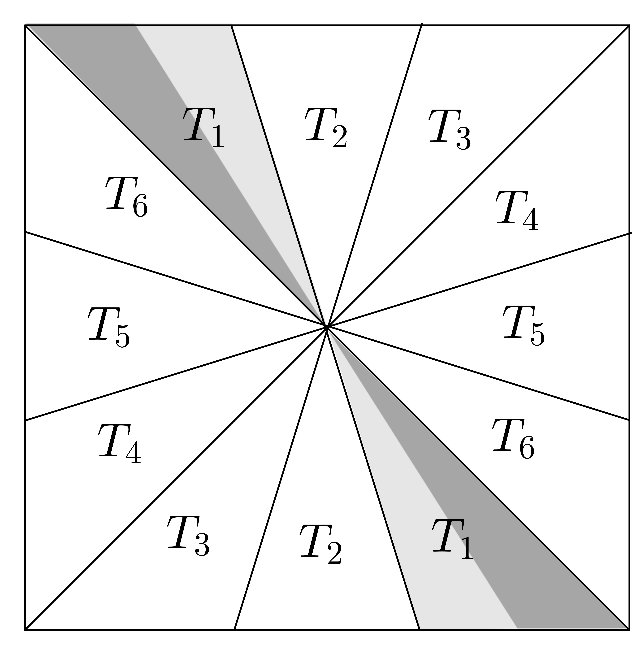
\includegraphics[width = .4\textwidth]{triangle-partition-new.png}
\caption{Partition of frequency square in six directions, where the essential support of $\m{i}$ is contained in each pair of triangles $T_i$. The pair of dark grey triangles is $T_1^-$ and the light grey pair is $T_1^+$.}
\label{fig: partition 2}
\end{figure}
%Let pairs of triangles $T_i$ in Fig.\ref{fig: partition 2} contain the essential support of $\widetilde{m_i},\,i=1,\cdots,6$.
%\eqref{eq: LS-new} takes a similar form to \eqref{eq: LS}, but with $\M\in\mathbb{C}^{8\times 7}$, which is an over-determinant linear system.
In what follows, we introduce a triangular partition of $S_0=[-\pi,\pi)\times[-\pi,\pi)$ in the frequency plane and define formally the concentration of the support of the $\widetilde{m_j}$.

\noindent{\bf Definition.}
The {\it  domination-support} $\Omega_j$ of a function $\widetilde{m_j}$ (with respect to the other $m_i$, $i\neq j$) is the set $\{\V{\omega}:\,|\widetilde{m_j}(\V{\omega})|> |\widetilde{m_i}(\V{\omega})|,\,\forall i\neq j\}$. \vspace{.5em}

Let $T_j$ be pairs of triangles shown in Figure \ref{fig: partition 2}, defined such that $C_j\subset T_j,\, j = 1,\cdots,6.$ Consider the decompositions $T_j = T_j^-\bigcup T_j^+$, where $T_j^-, T_j^+$ are halves of $T_j$ adjacent to its neighboring triangles $T_i$ in the counter clockwise and clockwise directions respectively.\\[.5em]
\noindent{\bf Definition.}  $\widetilde{m_j}$ {\it concentrates} within $T_j$ if 
\begin{itemize}
\item[(i)] $\Omega_j\subset T_j$;
\item[(ii)]$\text{supp}(\widetilde{m_j})\subset T_{j-1}^+\bigcup T_j\bigcup T_{j+1}^-$ and $\int_\Omega|\widetilde{m_j}| > \int_{\Omega'}|\widetilde{m_j}|, \forall\, \Omega\subset T_j\bigcap\text{supp}(\widetilde{m_j})$ s.t. $|\Omega|>0$, where $\Omega' \subset T_{j-1}^+\bigcup T_{j+1}^-$ is symmetric to $\Omega$ with respect to the boundary of $T_j$.
\end{itemize}
In other words, for $\widetilde{m_j}$ to concentrate in $T_j$, $\widetilde{m_j}$ should be ``mainly" supported in $T_j$ (condition (i)) and ``decay" properly outside of $T_j$ (condition (ii)).

\begin{figure}
\centering
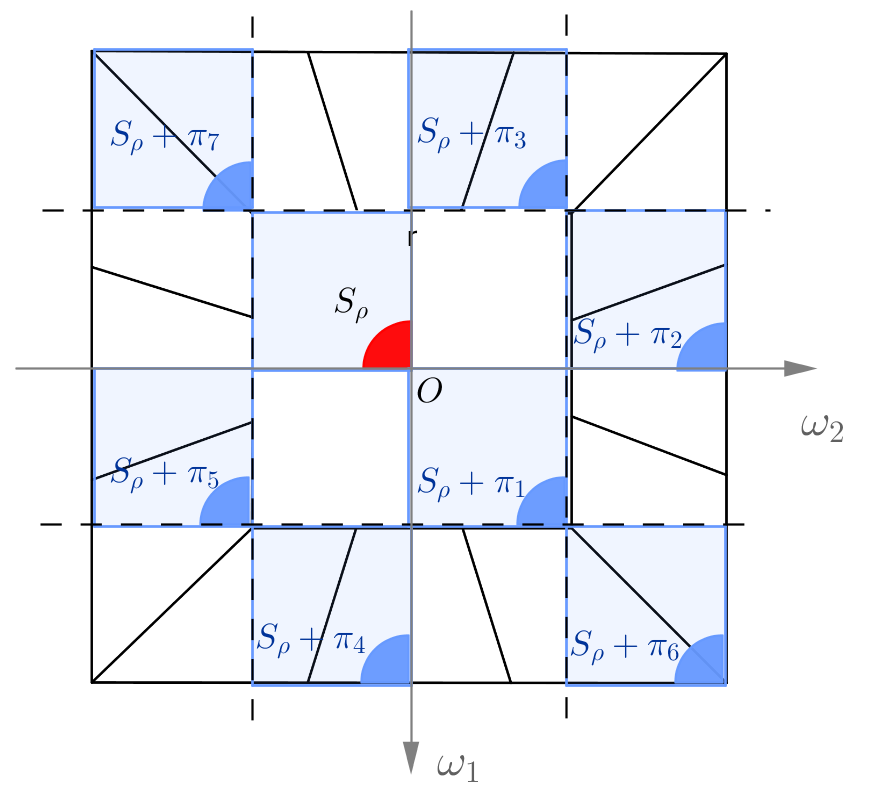
\includegraphics[width = .5\textwidth]{S_shifts2.png}
\caption{$S_{\rho}$ and its shifts}
\label{fig: S-shifts}
\end{figure}
Given $\m{j}$ that concentrates in $T_j$, we examine the consequences of the singularity condition on $\M[\widehat{0},:](\V{\omega})$ from Lemma \ref{lem: subM-singular}, specifically in the domain $S_{\rho} = \{(\omega_1,\omega_2)|\;\Vert\omega\Vert < \rho, \omega_1 <0,\,\omega_2<0\}$, see the red zone in Figure \ref{fig: S-shifts}. 

Let $\mrow{i}(\V{\omega}) = [\widetilde{m_1}(\V{\omega}+\V{\pi}_i)\, \cdots,\,\widetilde{m_6}(\V{\omega}+\V{\pi}_i)]\in\mathbb{C}^6,\, i = 0,\cdots,7$ be the rows of $\M[:,\widehat{0}](\V{\omega})$. 
\begin{lemma}\label{lem: rank1}
$\exists\, \rho>0$ s.t. if $\V{\omega}\in S_\rho$ and $\M[\widehat{0},:](\V{\omega})$ is singular, then $rank(\,\mrow{1}(\V{\omega}),\mrow{7}(\V{\omega})\,)=1$ or \\$rank(\,\mrow{3}(\V{\omega}\,),\mrow{5}(\V{\omega})) = 1$.
\end{lemma}
Lemma \ref{lem: rank1} can be proved by analyzing the linear dependency and independency between the $\mrow{i}$ on $S_\rho$, since the $\mrow{i}$ have known locations of zero entries when $\rho$ is small due to the concentration of the $\widetilde{m_j}$.
For the full proof of Lemma \ref{lem: rank1}, see Appendix \ref{app: lemmas}.

The concentration and the symmetry of $\m{3}$ and $\m{4}$ in $T_3$ and $T_4$ together imply that  $rank(\mrow{3},\mrow{5}) \neq 1\; a.e.$ on $S_\rho$, see Lemma \ref{lem: full-rank-m35} in Appendix \ref{app: discontinuity}, hence $rank(\,\mrow{1}(\V{\omega}),\mrow{7}(\V{\omega})\,) = 1\; a.e.$ on $S_\rho$.
Therefore, $\mp{1}{1}, \mp{6}{1}$ in $\mrow{1}(\V{\omega})$ and the corresponding $\mp{1}{7}, \mp{6}{7}$ in $\mrow{7}(\V{\omega})$ on $S_\rho$ are linearly related. Based on this and  the concentration and the symmetry of $\m{1}$ and $\m{6}$ in $T_1$ and $T_6$, we can show that $\m{1}=\m{6}=0\; a.e.$ on $S_\rho + \V{\pi}_1$, see Proposition \ref{prop: zero-corner} in Appendix \ref{app: discontinuity}, which implies the discontinuity of $\m{1}$ and $\m{6}$ at $(\frac{\pi}{2},\frac{\pi}{2})$ or $(-\frac{\pi}{2},-\frac{\pi}{2})$.

\begin{proposition}\label{prop: continuity}
Given the same condition as in Lemma \ref{lem: rank1}, $\m{1},\m{6}$ cannot be continuous at both $(\frac{\pi}{2},\frac{\pi}{2})$ and $(-\frac{\pi}{2},-\frac{\pi}{2})$.
\end{proposition}
\noindent{\it Proof. }
If $\m{1}$ is continuous at $(\frac{\pi}{2},\frac{\pi}{2})$, then $\widetilde{m_1}(\frac{\pi}{2},\frac{\pi}{2}) = \lim_{\alpha\rightarrow 1^-}\widetilde{m_1}(\V{\omega}(\alpha)) = 0$, where $\{\V{\omega}(\alpha),\,0\leq \alpha<1\} \subset S_\rho + \V{\pi}_1$ and $\V{\omega}(1) = (\frac{\pi}{2},\frac{\pi}{2})$. By symmetry, we have $\widetilde{m_6}(\frac{\pi}{2},\frac{\pi}{2}) = 0$. Similarly, the continuity at $(-\frac{\pi}{2},-\frac{\pi}{2})$ implies $\widetilde{m_1}(-\frac{\pi}{2},-\frac{\pi}{2}) = \widetilde{m_6}(-\frac{\pi}{2},-\frac{\pi}{2}) = 0$. Therefore $\mrow{1}(\V{0}) = \mrow{7}(\V{0}) = \mathbf{0}$ at the origin which results in contradiction with Lemma \ref{lem: rank1}.\qed\\[1em]%and from \eqref{eq: m0C} $m_0^C(0)=0$ so that $m_0(0)=0$, %  On the other hand, Proposition\ref{prop: origin-det} implies that $m_0(0) = 0$ as $a = |\widetilde{m_1}(\pi_1)| = 0$, which results in contradiction.
The following theorem summarizes our main result.
\begin{theorem}\label{thm: thm}
If the $\m{j}$ concentrate in $T_j$ and have symmetries \eqref{eq: sym-m16} and \eqref{eq: sym-m34}, then \eqref{eq: LS-new} doesn't have feasible solution of $m_j$ if $\m{1}$ and $\m{6}$ are continuous.
\end{theorem}

\section{Numerical construction of bi-orthogonal bases}\label{sec: solve-quincunx}
In this section, we develop a numerical construction of bi-orthogonal bases on a dyadic quincunx lattice following an approach similar to Cohen et al. We first design $\m{j},\,j = 1,\cdots,6,$ on the canonical frequency square $S_0 = [-\pi,\pi)\times[-\pi,\pi),$ then solve for $m_0,\widetilde{m_0}$ and $m_j$ on $S_0$ in order with respect to \eqref{eq: LS-new} and \eqref{eq: identity-cond}.
%we focus on solving $m_i$'s and $\widetilde{m_0}$ in \eqref{eq: LS-new} given pre-designed $\m{i},\,i=1,\cdots,6$. %Assume $\m{i},\,i=1,\cdots,6$ satisfy weak constraints on the direction selectivity of their support.

\subsection{Design of input $\m{j}$}\label{sec: phase-design}
In this sub-section, we construct $\m{j},\, j = 1,\cdots,6,$ which concentrate in $T_i$.
Specifically, following the orthonormal construction in \cite{yin2014orthshear}, we consider $\m{j}$ in the form 
\begin{align}\label{eq: m-form}
\m{j} = e^{-i\V{\eta}_j^\top\V{\omega}}|\m{j}|,\quad j = 1,\cdots,6,
\end{align}
where $\V{\eta}_j\in\mathbb{Z}^2$ is the phase constant of $\widetilde{m_j}$. In addition to the symmetry of pairs $(|\widetilde{m_1}|, |\widetilde{m_6}|)$ and $(|\widetilde{m_3}|, |\widetilde{m_4}|)$ assumed in Section \ref{subsec: discontinuity}, we further request that $|\widetilde{m_2}|$ and $|\widetilde{m_5}|$ are symmetric with respect to the $\omega_1$-axis and $\omega_2$-axis accordingly.
% where $|\m{j}|$'s have symmetries with respect to the two diagonals and the two axis. 
Figure \ref{fig: mjdual} shows such a design of $|\m{j}|$ that has the imposed strong symmetries.
 
Based on \eqref{eq: m-form} and the symmetries of $|\m{j}|$, for $|m_0(\V{\omega})| > 0,\, \forall\, |\V{\omega}| < \rho$, $\V{\eta}_j$ have to satisfy certain constraints.
% We want to design the phase $\V{\eta}_k$ such that $m_0(\V{\omega}) > 0, \; \forall \omega\in S_1$. This is the same as requiring $\Msub$ to be full rank. We first show the necessary conditions on phases $\V{\eta}$ of the full rank requirement on $\Msub$.
 
\begin{lemma}\label{lem: phase-ineq}
If $\exists\,\V{\omega}\in D_1:=\{\omega_1=\omega_2,\,\omega_1\in(-\frac{\pi}{2},0)\},\,s.t. \,|m_0(\V{\omega})|\neq 0,$ then $(\V{\eta}_1-\V{\eta}_6)^\top (\V{\pi}_6-\V{\pi}_7)\neq 0(\text{mod}\,2\pi)$. 
\end{lemma} 

Because $m_0(\V{\omega})$ can be expressed as in \eqref{eq: m0-cramer}, $|m_0(\V{\omega})|\neq 0$ is equivalent to $\det(\,\Msub[\widehat{k_{\V{\omega}}},:](\V{\omega})\,)\neq 0$, i.e. $\Msub(\V{\omega})$ is full rank. The constraint on $\V{\eta}_1$ and $\V{\eta}_6$ then follows from substituting non-zero entries of $\Msub(\V{\omega})$ by \eqref{eq: m-form} and consider the linear dependency of the columns in $\Msub(\V{\omega})$. For the full proof of Lemma \ref{lem: phase-ineq}, see Appendix \ref{app: input design}.

Similarly, if $\exists\,\V{\omega}\in \{\omega_1 = \omega_2,\, \omega_1\in(0,\frac{\pi}{2})\},\, s.t.\, |m_0(\V{\omega})| \neq 0$, then $(\V{\eta}_1-\V{\eta}_6)^\top (\V{\pi}_6-\V{\pi}_1)\neq 0(\text{mod}\,2\pi)$. These two conditions are equivalent to 
\begin{align*}
(\V{\eta}_1-\V{\eta}_6)^\top(\pi/2,\pi/2)\neq 0 (\text{mod}\,2\pi)\tag{\bf c1.1}
\end{align*}
since $\V{\eta}_1,\,\V{\eta}_6\in\mathbb{Z}^2$.
Considering the other diagonal segment $\{\omega_2 = -\omega_1, |\omega_1| <\frac{\pi}{2}\}$, we also have 
\begin{align*}
(\V{\eta}_3-\V{\eta}_4)^\top(-\pi/2,\pi/2)\neq 0 (\text{mod}\, 2\pi)\tag{\bf c1.2}
\end{align*}
%from the full rank condition.

Next, we consider $\widetilde{m_0}(\V{0})$ and investigate $\Msub(\V{\omega})$ at the origin.
\begin{proposition}\label{prop: origin-det}
%If $|\widetilde{m_1}(\V{\pi}_1)| = |\widetilde{m_1}(\V{\pi}_7)| = |\widetilde{m_3}(\V{\pi}_3)| = |\widetilde{m_3}(\V{\pi}_5)|$ and $|\widetilde{m_1}(\V{\pi}_6)|= | \widetilde{m_3}(\V{\pi}_6)|$, then 
If $|\widetilde{m_0}(\V{0})|\neq 0,$ then $\V{\pi}_1^\top(\V{\eta}_1-\V{\eta}_6)\neq \pi(\text{mod}\,2\pi)$ or $\V{\pi}_3^\top(\V{\eta}_3-\V{\eta}_4)\neq \pi(\text{mod}\,2\pi)$. 
\end{proposition}
\noindent{\it Remark.}
The proof of Proposition \ref{prop: origin-det} is similar to that of Lemma \ref{lem: phase-ineq} but more involved. See Appendix \ref{app: input design} for the full proof.

\begin{comment}
{\it Remark.} In Lemma \ref{lem: phase-ineq}, $\Msub[:,1]$ and $\Msub[:,6]$ being independent only guarantees $\det(\Msub[\widehat{k_{\V{\omega}}},:])\neq 0$. However, \eqref{eq: m0-cramer} implies that $|m_0(\V{\omega})|\propto \det(\Msub[\widehat{k_{\V{\omega}}},:])$ hence it is preferred to maximize the determinant. Since
\begin{align*}
\det(\Msub[\widehat{k_{\V{\omega}}}, :]) = \det\big(\big[\, \Msub[\widehat{k_{\V{\omega}}},-6], \;\Msub[\widehat{k_{\V{\omega}}},6] + c \cdot\Msub[\widehat{k_{\V{\omega}}},1]  \,\big]\big),\quad 
\end{align*}
$\forall c\in \mathbb{C}$, the angle between $\Msub[:,1]$ and $\Msub[:,6]$ should be maximized.
Therefore, a stronger condition than ({\bf c1.1}) is to require $\Msub[:,1]$ and $\Msub[:,6]$ be orthogonal, which is equivalent to 
\begin{align*}
(\V{\eta}_1-\V{\eta}_6)^\top(\pi/2, \pi/2) = \pi \,(\text{mod}\, 2\pi).\tag{\bf c2.1}
\end{align*}
The stronger condition corresponding to ({\bf c1.2}) is 
\begin{align*}
(\V{\eta}_3-\V{\eta}_4)^\top(-\pi/2,\pi/2)=\pi(\text{mod},\,2\pi).\tag{\bf c2.2}
\end{align*} %from the stronger orthogonal condition.

%{\it Remark}
%f $|\m{1}| = |\m{2}|$ on $\{\omega_y = 3\omega_x,\,|\omega_x| > \frac{\pi}{2}\}$ and $m_0(\V{\omega}) > 0$ on $\{\omega_y = 3\omega_x\pm \pi,\,|\omega_y| <\frac{\pi}{2}\}$, then the same conditions ({\bf c1}) and ({\bf c2}) can be derived from full rank and orthogonal conditions respectively for tuples $(\,\V{\eta}_1,\,\V{\eta}_2,(-\pi/2,\pi/2)\,),\,(\,\V{\eta}_2,\V{\eta}_3,(\pi/2,\pi/2)\,),\,(\V{\eta}_4,\V{\eta}_5,\,(\pi/2,\pi/2)\,)$ and $(\,\V{\eta}_5,\V{\eta}_6,\,(-\pi/2,\pi/2)\,)$. 

% If the previous strong orthogonal condition on $\V{\eta}_1, \V{\eta}_3, \V{\eta}_4,\V{\eta}_6$ holds, then $K_1 = K_2 = 0$ and $m_0(0)=m_0^C(0)= 0$. Therefore, the strong orthogonal conditions ({\bf c2}) cannot be satisfied at the same time. 
%In particular, we consider the following constraints on phase $\V{\eta}_k\in \mathbb{Z}^2,\, k = 1,\cdots,6$:
Unfortunately, Proposition \ref{prop: origin-det} prevents ({\bf c2.1}) and ({\bf c2.2}) from holding simultaneously.
\end{comment}
We propose the following set of phases such that ({\bf c1.1}) and ({\bf c1.2}) as well as the necessary condition from Proposition \ref{prop: origin-det} are all satisfied,
\begin{align}\label{eq: phase-sol}
\V{\eta}_1 = (0,0),\; \V{\eta}_2 = (-1,1),\; \V{\eta}_3 = (0,2),\notag\\
\V{\eta}_4 = (1,0),\; \V{\eta}_5 = (0,-1),\; \V{\eta}_6 = (0,1).
\end{align}
\begin{comment}
where
\begin{align*}
%\label{eq: phase-constraint}
%&(\V{\eta}_1-\V{\eta}_2)^\top(-\pi/2, \pi/2) = (\V{\eta}_5-\V{\eta}_6)^\top(-\pi/2,\pi/2) = \pi\, (\text{mod}\, 2\pi)\notag\\
%&(\V{\eta}_2-\V{\eta}_3)^\top(\pi/2,\pi/2) = (\V{\eta}_4-\V{\eta}_5)^\top(\pi/2,\pi/2) = \pi\, (\text{mod}\, 2\pi)\\
%&
(\V{\eta}_3-\V{\eta}_4)^\top(-\pi/2, \pi/2) &=-\pi/2\,(\text{mod}\,2\pi)\notag\\
 (\V{\eta}_6 - \V{\eta}_1)^\top(\pi/2,\pi/2) &= \pi/2\, (\text{mod}\,2\pi)\notag
\end{align*}
%where we require strong orthogonal constraints on pair of shifts corresponding to $\widetilde{m}$ function with non-diagonal common boundary and weaker constraints on $(\V{\eta}_1,\V{\eta}_6)$ and $(\V{\eta}_3,\V{\eta}_4)$. A solution to \eqref{eq: phase-constraint} is 
\end{comment}

\subsection{Solving \eqref{eq: LS-new} and \eqref{eq: identity-cond} for $m_0,\widetilde{m_0}$ and $m_j$}\label{subsec: compute-m0}
Once $\m{j}, j= 1,\cdots, 6$ are fixed on $S_0$, \eqref{eq: LS-new} can be reformulated as follows,
\begin{align}\label{eq: mj-eq}
\M[:,\widehat{0}](\V{\omega}) 
\begin{bmatrix}
m_1(\V{\omega})\\
m_2(\V{\omega})\\
m_3(\V{\omega})\\
m_4(\V{\omega})\\
m_5(\V{\omega})\\
m_6(\V{\omega})
\end{bmatrix}
= \V{b}_0 - m_0(\V{\omega})
\begin{bmatrix}
 \sbarm{0}\\
 0\\
\sbarmp{0}{2}\\
0\\
\sbarmp{0}{4}\\
0\\
\sbarmp{0}{6}\\
0
\end{bmatrix} \doteq \V{b}_0'(\V{\omega}),
\end{align}
where $\M[:,\widehat{0}](\V{\omega})$ is completely determined by $\m{j},\,j = 1,\cdots,6$ 
and $m_j,\,j=1,\cdots,6$ can be uniquely solved on $S_0$ if and only if $\forall\V{\omega}\in S_0$
\hspace{-1em}
\begin{enumerate}[leftmargin=.5in]
\item[\mylabel{cond: i}{(\ref{subsec: compute-m0}.i)}] $\M[:,\widehat{0}](\V{\omega})$ is full rank,%
\item[\mylabel{cond: ii}{(\ref{subsec: compute-m0}.ii)}] $\V{b}_0'(\V{\omega})$ is in $col\big(\M[:,\widehat{0}](\V{\omega})\big)$, the column space of $\M[:,\widehat{0}](\V{\omega})$.%
\end{enumerate}
%Because , \ref{cond: i} can be easily checked by computing $\det(\M[:,\widehat{0}]^\top\M[:,\widehat{0}])$ and see if it is non-zero. Next, we show that (ii) provides an explicit way of computing $m_0(\V{\omega})$ without knowing $\m{0}$.
Next, we show that \ref{cond: ii} breaks down to constraints on two submatrices of $\M[:,\widehat{0}](\V{\omega})$ and quadruples $\big( m_0(\V{\omega}),m_0(\V{\omega}+\V{\pi}_2), m_0(\V{\omega} +\V{\pi}_4), m_0(\V{\omega}+\V{\pi}_6) \big)$, $\big( m_0(\V{\omega}+\V{\pi}_1),m_0(\V{\omega}+\V{\pi}_3), m_0(\V{\omega} +\V{\pi}_5), m_0(\V{\omega}+\V{\pi}_7) \big)$.
\begin{proposition}\label{prop: m0_formula}
Let $\M[odd,\widehat{0}](\V{\omega}),\M[even,\widehat{0}](\V{\omega})\in\mathbb{C}^{4\times6}$ be the sub-matrices of $\M[:,\widehat{0}](\V{\omega})$ consisting of odd and even indexed rows respectively. $\forall\V{\omega}\in S_0$, suppose {\rm\ref{cond: i}} holds, then {\rm\ref{cond: ii}} holds if and only if $rank(\,\M[odd,\widehat{0}](\V{\omega})\,) = rank(\,\M[even,\widehat{0}](\V{\omega})\,) = 3$ and 
\begin{align}\label{eq: m0-even-null}
[m_0(\V{\omega}),m_0(\V{\omega}+\V{\pi}_2), m_0(\V{\omega} +\V{\pi}_4), m_0(\V{\omega}+\V{\pi}_6)]\, \M[even,\widehat{0}](\V{\omega}) = \V{0},
\end{align}
\begin{align}\label{eq: m0-odd-null}
[m_0(\V{\omega}+\V{\pi}_1),m_0(\V{\omega}+\V{\pi}_3), m_0(\V{\omega} +\V{\pi}_5), m_0(\V{\omega}+\V{\pi}_7)] \,\M[odd,\widehat{0}](\V{\omega}) = \V{0}.
\end{align}
\end{proposition}

For the proof of Proposition \ref{prop: m0_formula}, see Appendix \ref{app: solving}.

\noindent{\it Remark.} 
Note that the submatrices $\M[odd,\widehat{0}](\V{\omega})$ and $\M[even,\widehat{0}](\V{\omega})$ are dual to each other under the shift of variable $\V{\omega}\mapsto \V{\omega}+\V{\pi}_i$, when $i$ is odd. Therefore, the constraints $rank(\,\M[even,\widehat{0}](\V{\omega})\,) = 3$ and \eqref{eq: m0-even-null} from Proposition \ref{prop: m0_formula} are sufficient for \ref{cond: ii} to hold on $S_0$. Furthermore, because $\M[even, \widehat{0}](\V{\omega})$ and $(\V{\omega},\V{\omega}+\V{\pi}_2,\V{\omega}+\V{\pi}_4, \V{\omega} + \V{\pi}_6)$ are invariant to the shift of variable $\V{\omega}\mapsto\V{\omega}+\V{\pi}_i$ when $i$ is even, we only need to consider the constraints above on the subset $[-\pi,0)\times[-\pi,0)$ of $S_0$.
%Both conditions \eqref{eq: m0-even-null} and \eqref{eq: m0-odd-null} hold $\forall \V{\omega}\in[-\pi,\pi)\times[-\pi,\pi)$ if and only if \eqref{eq: m0-even-null} holds $\forall \V{\omega}\in [-\pi,0)\times[-\pi,0)$.

In sum, $\M[:,\widehat{0}](\V{\omega})$ (or equivalently $\widetilde{m_j}$) has to satisfy the following rank constraints on $[-\pi,0)\times[-\pi,0)$ for \eqref{eq: mj-eq} to be uniquely solvable on $S_0$, 
\begin{align}\label{eq: Mranks}
rank(\,\M[:,\widehat{0}](\V{\omega})\,) = 6,\, rank(\,\M[even,\widehat{0}](\V{\omega})\,) = 3.
\end{align}
As the rank constraints are hard to impose while designing $\widetilde{m_j}$, in our numerical experiments, we check if these rank constraints are satisfied afterwards, see step 1. in \ref{alg}.

Suppose \eqref{eq: Mranks} hold, the quadruple  $\big( m_0(\V{\omega}),m_0(\V{\omega}+\V{\pi}_2), m_0(\V{\omega} +\V{\pi}_4), m_0(\V{\omega}+\V{\pi}_6) \big)$ can then be uniquely determined by \eqref{eq: m0-even-null} {\it up to a constant $a_{\V{\omega}} $}, where its corresponding vector is orthogonal to the column space of $\M[even,\widehat{0}](\V{\omega})$ of co-dimension 1. In particular, we obtain $m_0(\V{\omega})$ on $S_0$ by solving \eqref{eq: m0-even-null} independently at each $\V{\omega}$ on $[-\pi,0)\times[-\pi,0)$, see step 2. in \ref{alg}. Since the constant $a_{\V{\omega}}$ can change drastically as $\V{\omega}$ changes, there is potential lack of regularity of $m_0(\V{\omega})$ as an artifact of the algorithm. Figure \ref{fig: m_0_m0dual} shows an $m_0(\V{\omega})$ computed in this way, which has discontinuous phase due to $a_{\V{\omega}}$. Fortunately, this artificial irregularity can be removed as suggested by the following proposition.

\begin{comment}
By Lemma \ref{lem: M-symmetry}, $\M[:,\widehat{0}]$ are the same at $\V{\omega},\V{\omega}+\V{\pi}_2,\V{\omega}+\V{\pi}_4$ and $\V{\omega} + \V{\pi}_6$ up to row permutations. Therefore, the columns of the matrix $\V{B}$ below should be in $col\big(\M[:,\widehat{0}](\V{\omega})\big)$,
\begin{align*}
\V{B}&= \widetilde{\mathbf{m}_0}^\uparrow\otimes\mathbf{m}_0 - [\V{b}_0,\V{b}_2,\V{b}_4,\V{b}_6]\\
&\doteq
\begin{bmatrix}
 \overline{\widetilde{m_0}}(\V{\omega})\\
 0\\
\sbarmp{0}{2}\\
0\\
\sbarmp{0}{4}\\
0\\
\sbarmp{0}{6}\\
0
\end{bmatrix}
\otimes
\begin{bmatrix}
 m_0(\V{\omega})\\
 m_0(\V{\omega} + \V{\pi}_2)\\
 m_0(\V{\omega} + \V{\pi}_4)\\
 m_0(\V{\omega} + \V{\pi}_6) 
\end{bmatrix}
-
\begin{bmatrix}
1 & 0 & 0 & 0\\
0 & 0 & 0 & 0\\
0 & 1 & 0 & 0\\
0 & 0 & 0 & 0\\
0 & 0 & 1 & 0\\
0 & 0 & 0 & 0\\
0 & 0 & 0 & 1\\
0 & 0 & 0 & 0
\end{bmatrix},
\end{align*}

Let $\M[:,\widehat{0}] = U\Sigma V^\top$ be the singular value decomposition of $\M[:,\widehat{0}]$, such that $U(\V{\omega})\in\mathbb{C}^{8\times 6}$ consists of left singular vectors of $\M[:,\widehat{0}](\V{\omega})$ and $UU^\top(\V{\omega})$ is a projection matrix of $col\big(\M[:,\widehat{0}](\V{\omega})\big)$. Therefore, $\V{B}$ satisfies
\begin{align}\label{eq: cond-full}
\V{P}\V{B} = (\V{U}\V{U}^\top - \V{I}_8 )\V{B} = \V{0}\in\mathbb{C}^8,
\end{align}
 where $\V{P}$ is the projection onto $col\big(\M[:,\widehat{0}](\V{\omega})\big)^\bot$, $\V{I}_8$ is the identity matrix in $\mathbb{C}^8$. Because the even rows of $\V{B}$ are all zeros, we can down-sample its rows and correspondingly the columns of $\V{P}$ and \eqref{eq: cond-full} can be reduced to 
\begin{align}
\V{P}^\downarrow\V{B}^\downarrow = \V{P}^\downarrow \big(\widetilde{\mathbf{m}_0}\otimes \mathbf{m}_0 - \V{I}_4\big) = \V{0}\in\mathbb{C}^8
\end{align}
$\V{P}^\downarrow\in\mathbb{C}^{8\times 4}$ consists of odd columns of $\V{P}$ and $\V{B}^\downarrow\in\mathbb{C}^{4\times 4}$ consists of odd rows of $\V{B}$.

Let $C_{\V{\omega}} = det(\M[\widehat{k_{\V{\omega}}},:])$, then we have the following observation.
\begin{lemma}\label{lem: equal-det}
$C_{\V{\omega}} = C_{\V{\omega}+\V{\pi}_2} = C_{\V{\omega}+\V{\pi}_4} = C_{\V{\omega}+\V{\pi}_6}$
\end{lemma}
\noindent{\it Proof}
Because $\widetilde{M}(\V{\omega}+\V{\pi}_2) = P_{\V{\pi}_2}\M(\V{\omega})$ where $P_{\V{\pi}_2}$ is a row permutation matrix, it follows from the definition of $C_{\V{\omega}}$ that 
$C_{\V{\omega}} = det\big(\M[\widehat{k_{\V{\omega}}},:](\V{\omega})\big) = det\big(\M[-k_{\V{\omega}+\V{\pi}_2},:](\V{\omega}+\V{\pi}_2) \big)= C_{\V{\omega}+\V{\pi}_2}$ where 
$\mathbf{1}_{k_{\V{\omega}+\V{\pi}_2}} = P_{\V{\pi}_2}\mathbf{1}_{\widehat{k_{\V{\omega}}}}$.
\qed\\[1em]
We assume that $m_0\in\mathbb{R}_{\geq 0}$ without phase. Let $m_0^C(\V{\omega}) = m_0(\V{\omega})|C_{\V{\omega}}|\in \mathbb{R}_{\geq 0}$ and $\mc{0} = \m{0}/|C_{\V{\omega}}|$, then Lemma \ref{lem: equal-det} implies the following.
\end{comment}


\begin{proposition}\label{prop: mc}
If $\m{j}, m_j(\V{\omega}),\,  j = 0,1,...,6$ satisfy \eqref{eq: LS-new} and \eqref{eq: identity-cond}, 
%$m_0^C(\V{\omega}),$ $\,\mc{0}, m_i(\V{\omega}),\,i = 1,...,6$ do. More generally, 
%$m_0(\V{\omega})c(\V{\omega}),\,\m{0}c(\V{\omega})^{-1}, m_i(\V{\omega}),\,i=1,...,6$ 
then $m_0'(\V{\omega})\doteq m_0(\V{\omega})c(\V{\omega}), \widetilde{m_0}'(\V{\omega})\doteq \m{0}\overlinespace{c}(\V{\omega})^{-1}$ together with the same $m_j(\V{\omega}),\m{j}, \, j = 1,\cdots,6$ 
satisfy \eqref{eq: LS-new} and \eqref{eq: identity-cond} if $ c(\V{\omega}) = c(\V{\omega}+\V{\pi}_2)=c(\V{\omega}+\V{\pi}_4) = c(\V{\omega}+\V{\pi}_6) \neq 0$, i.e. $c(\V{\omega})$ is $\pi$-periodic in both $\omega_1$ and $\omega_2$.
\end{proposition}
\noindent{\it Proof. }
It suffices to show that $m_0'(\V{\omega})\overline{\widetilde{m_0}'}(\V{\omega} + \V{\pi}_i) = m_0(\V{\omega})\sbarmp{0}{i},\,$ when $i$ is even.\qed

%\begin{align*}
%m_0^c(\V{\omega})\overline{\widetilde{m_0}^c}(\V{\omega} + \V{\pi}_i) = m_0(\V{\omega})\sbarmp{0}{i},\quad & i \text{ is even,}\hspace{4em}\qed
%\hspace{1em}m_j^c(\V{\omega})\overline{\widetilde{m_j}^c}(\V{\omega} + \V{\pi}_i) = \big(m_j(\V{\omega})\sbarmp{j}{i}\big)c(\V{\omega})c(\V{\omega}+\V{\pi}_1)^{-1},\quad & i \text{ is odd.}\qedhere\hspace{2em}\qed
%\end{align*}

\noindent{\it Remark.}
Proposition \ref{prop: mc} suggests that we can compensate $a_{\V{\omega}}$ by choosing $c(\V{\omega})$ such that $(m_0',\widetilde{m_0}')$ have improved regularity, e.g. continuity, smoothness or fast decay rate. In practice, we first solve $\m{0}$, step 3. in \ref{alg}, then choose $c(\V{\omega})$ $\pi$-periodic in both axis and replace $m_0(\V{\omega})$ and $\widetilde{m_0}(\V{\omega})$ by $m_0'(\V{\omega})$ and $\overline{\widetilde{m_0}'}(\V{\omega})$ as defined in Proposition \ref{prop: mc}.

To obtain $\m{0}$ on $S_0$, we solve the identity condition \eqref{eq: identity-cond} on $[-\pi, 0)\times[-\pi, 0 )$ for the quadruple $(\m{0}, \mp{0}{2}, \mp{0}{4}, \mp{0}{6})$. Note that \eqref{eq: identity-cond} is the same as \eqref{eq: bi-orth-eq} in Section \ref{subsec: cohen-summary}. 
According to Lemma 3.2.1 in \cite{cohen1993compactly}, based on {\it Hilbert's Nullstellensatz}, \eqref{eq: bi-orth-eq} has a solution if and only if there does not exist $(z_1,z_2)\in (\mathbb{C}^*)^2,\, \mathbb{C}^* = \mathbb{C}\setminus\{0\}$\, s.t. $(\pm z_1,\pm z_2)$ are all vanishing points of the $z$-transform of $m_0$.
In general, there is no efficient algorithm to solve {\it Hilbert's Nullstellensatz}, and how \eqref{eq: bi-orth-eq} is solved exactly is not mentioned in \cite{cohen1993compactly}.
%In Section \ref{sec: numerics}, we propose an optimization problem that solves $\widetilde{m_0}$, where \eqref{eq: m0-sol} (which is the same as \eqref{eq: identity-cond}) serves as a linear constraint.
%As mentioned at the end of Section \ref{subsec: cohen-summary}, we are not aware of existing efficient algorithms that solve \eqref{eq: identity-cond}. 

Here, we reformulate it as an optimization problem wher \eqref{eq: identity-cond} serves as a linear constraint. In particular, on a $2N\times 2N$ regular grid $\G=\{\V{\omega}_i\}_{i=1}^{4N^2}$ of $[-\pi, \pi)\times[-\pi, \pi), $ \eqref{eq: identity-cond} can be rewritten as
\begin{align}
\V{A}\, \overlinespace{\widetilde{\mathbf{m}_0}}= \mathbf{1}_{4N^2}, \label{eq: m0-A}%\\ 
%\widetilde{\mathbf{m}_0} = [\widetilde{m_0}(\V{\omega}_i)]_{\,i=1,\hdots,4N^2}&\in\mathbb{C}^{4N^2} \notag
\end{align}
where $\widetilde{\mathbf{m}_0} = [\widetilde{m_0}(\V{\omega}_i)]_{\,i=1}^{4N^2}$ and $\V{A}\in \mathbb{C}^{N^2\times 4N^2}$ is a sparse matrix with entries 
$$\V{A}_{i,j} = m_0(\V{\omega}_j)\sum_{k=0}^3\delta(\V{\omega}_j-\V{\omega}_i-\V{\pi}_{2k}), \quad \V{\omega}_j \in [-\pi,0)\times[-\pi,0).$$

We optimize the regularity of $\sbarm{0}m_0(\V{\omega})$ instead of $\sbarm{0}$, as this product remains the same for $(\,m_0'(\V{\omega}), \widetilde{m_0}'(\V{\omega})\,)$ and its regularity controls the regularity of $(\,m_0'(\V{\omega}), \widetilde{m_0}'(\V{\omega})\,)$ that can be achieved.
We choose the squared $\ell_2$ norm of the gradient of $\sbarm{0}m_0(\V{\omega})$ as the objective function, although other forms of regularity may be imposed by different objective functions.

In sum, we solve the following quadratic minimization problem with linear constraint,
%On a $2N\times 2N$ grid $\G$ of $S_0 = [-\pi, \pi)\times[-\pi, \pi)$, s.t. $\forall \V{\omega}_j \in \G, \; \V{\omega}_j+\V{\nu}_1,\,\V{\omega}_j+\V{\nu}_2,\,\V{\omega}_j+\V{\nu}_3 \in \G$, \eqref{eq: m0-sol} is reformulated as
\begin{align}\label{eq: opt}
\min_{\xvec}\; \Vert \V{D}(\mathbf{m}_0\circ\xvec)\Vert^2,\quad 
s.t. \; \V{A}\xvec = \mathbf{1},
\end{align}
where $\V{D}$ is the gradient operator, $\circ$ is Hadamard product and $\V{A}$ is the linear operator from \eqref{eq: identity-cond}. 
%Because the set $\{\V{\omega},\, \V{\omega}+\V{\nu}_k,k=1,2,3\}$ is invariant under the shift $\V{\nu}_i,\, i = 1,2,3,$ the rows of $\V{A}$ corresponding to $\V{\omega}$ and $\V{\omega}+\V{\nu}_i$ are identical and 
%Because we only need to consider \eqref{eq: identity-cond} on $[-\pi,0)\times[-\pi,0)$, 
%rows corresponds to $\V{\omega}\in [-\pi,\pi)\times[-\pi,\pi)/\{\V{0},\,\V{\nu}_i,i=1,2,3\}$. Therefore, after removing the duplicate rows, 
%$\V{A}\in \mathbb{C}^{N^2\times 4N^2}$ and \eqref{eq: m0-A} is under-determinant. \\
%We thus use \eqref{eq: m0-A} as a linear constraint in quadratic optimization to solve $\mathbf{\widetilde{m}_0}$. Suppose that $\m{0}$ is smooth, then we build a differential operator $\V{D}$ and solve the following minimization problem:
%or
%\begin{align}
%&\min_{\mvec{0}}\; \Vert \V{D}\mvec{0}\Vert^2 + \lambda \Vert \V{A}\mvec{0} - \mathbf{1}\Vert^2 \label{eq: m0-smooth-relaxed}
%\end{align}
%The solution of \eqref{eq: m0-smooth-relaxed} is $\mvec{0} = \lambda(\lambda \V{A}^\top \V{A} + \V{D}^\top \V{D})^{-1}\V{A}^\top\mathbf{1}$.

%Or suppose $\m{0}$ decays away from the origin, then we build a diagonal weighting operator $\V{W}$, and solve the following minimization problem:
%\begin{align}\label{eq: opt-weight}
%&\min_{\mvec{0}}\; \Vert \V{W}\mvec{0}\Vert^2,\quad s.t. \; \V{A}\mvec{0} = \mathbf{1}
%\end{align}
Supplementary numerical results on solving $\m{0}$ by optimization are provided in Appendix \ref{app: supp-numerical}, where we test this optimization method on known bi-orthogonal filters $m_0$ and $\widetilde{m_0}$ and compare the solution from the optimization with the ground truth.

Finally, we plug $m_0(\V{\omega})$ and $\m{0}$ into $\V{b}_0'(\V{\omega})$ on the right of \eqref{eq: mj-eq} and solve the linear system, which has a guaranteed unique solution.

%According to Proposition \ref{prop: mc}, we can first solve $\mc{0}$ and $m_0^C(\V{\omega})$ and then construct $c(\V{\omega})$ for optimal $\m{0}$ and $m_0(\V{\omega})$. 
%In particular, $m_0^C$ can be computed without knowing $\widehat{k_{\V{\omega}}}$,
%\begin{align}\label{eq: m0C}
%m_0^C(\V{\omega}) = m_0(\V{\omega})|C_{\V{\omega}}| = |det(\M_{1,1}[\widehat{k_{\V{\omega}}},:])| = \prod_{i=1}^6\sigma_i(\M_{1,1}[\widehat{k_{\V{\omega}}},:]) = \prod_{i=1}^6\sigma_i(\M_{1,1}).
%\end{align}
%In practice, we first perform QR decomposition on $\Msub:=\M_{1,1}$ and then take the absolute value of the product of the diagonal entries of the upper triangular matrix, $diag(R)$. 
\vspace{.5em}
\noindent\begin{minipage}{\linewidth}
\rule{\textwidth}{.5pt}
\vspace*{-2em}
\begin{description}% prevent items from splitting
\item[\mylabel{alg}{Algorithm 1}. Construction of $m_0,\widetilde{m_0}$ and $\widetilde{m_j}$ in bi-orthogonal basis]\
\begin{itemize}
\item[Input:] $\m{j},\,j=1,...,6$
\item[step 1.] construct $\M[:,\widehat{0}](\V{\omega})$ on sub-grid $[-\pi,0)\times[-\pi,0)$ and check rank constraints \eqref{eq: Mranks},%compute $m_0^C(\V{\omega}) = \left|det(\M_{1,1}[\widehat{k_{\V{\omega}}},:])\right|$
\item[step 2.] solve quadruple $\big( m_0(\V{\omega}),m_0(\V{\omega}+\V{\pi}_2), m_0(\V{\omega} +\V{\pi}_4), m_0(\V{\omega}+\V{\pi}_6) \big)$ using \eqref{eq: m0-even-null} on $[-\pi,0)\times[-\pi,0)$,%compute $\mc{0}$, such that \eqref{eq: LS-new} is solvable and \eqref{eq: identity-cond} holds
\item[step 3.] solve the optimization \eqref{eq: opt} for $\m{0}$ on grid $[-\pi,\pi)\times[-\pi,\pi)$,
\item[step 4.] choose $\pi$-periodic $c(\V{\omega})$ and replace $m_0(\V{\omega}),\, \m{0}$ by $m_0'(\V{\omega}) = c(\V{\omega})m_0(\V{\omega})$ and $\widetilde{m_0}'(\V{\omega})=\m{0}\overline{c}(\V{\omega})^{-1}$,
%solve $m_i(\V{\omega}),\, i=1,...,6$ according to \eqref{eq: LS-new}
\item[step 5.] solve the reduced linear system \eqref{eq: mj-eq} for $m_j(\V{\omega}),\, j = 1,\cdots,6$.%design $c(\V{\omega})$ and let $m_0(\V{\omega}) = m_0^C(\V{\omega})c(\V{\omega}),\,\m{0} = \mc{0}\overline{c}(\V{\omega})^{-1}$
\end{itemize}
\end{description}
\vspace*{-1em}
\rule{\textwidth}{.5pt}
\end{minipage}\\[.5em]
To sum up, we propose \ref{alg} for bi-orthogonal directional filter construction with dyadic quincunx downsampling scheme.

\noindent{\it Remark.}
The order of step 4. and step 5. in \ref{alg} can be reversed because \eqref{eq: mj-eq} only depends on $m_0(\V{\omega})\overline{\widetilde{m_0}}(\V{\omega} + \V{\pi}_i)$ when $i$ is even, which remains the same for $m_0'(\V{\omega}),\widetilde{m_0}'(\V{\omega})$ regardless of $c(\V{\omega})$ by construction.

It is not necessary, but we may also manipulate pairs of $(m_j,\widetilde{m_j})$ according to the following generalization of Proposition \ref{prop: mc}.
\begin{proposition}\label{prop: mjc}
If $\m{j}, m_j(\V{\omega}),\,  j = 0,1,...,6$ satisfy \eqref{eq: LS-new} and \eqref{eq: identity-cond}, 
$m_j^c(\V{\omega})\doteq m_j(\V{\omega})c_j(\V{\omega}), \widetilde{m_j}^c(\V{\omega})\doteq \m{j}\overlinespace{c_j}(\V{\omega})^{-1} \, j = 0,\cdots,6$ 
satisfy \eqref{eq: LS-new} and \eqref{eq: identity-cond} if $ c_0(\V{\omega}) = c_0(\V{\omega}+\V{\pi}_{2k})\,,\forall k = 0,\cdots,3$ and $c_j(\V{\omega}) = c_j(\V{\omega} + \V{\pi}_k),\, \forall \;k = 0,\cdots,7,\, j = 1,\cdots,6$.
\end{proposition}

\begin{comment}
\subsection{solving $m_i$}
In the final step, we substitute $\mc{0}$ and $m_0^C(\V{\omega})$ into \eqref{eq: LS-new} and rewrite it into the following linear system,
\begin{align}\label{eq: mi}
\overline{\M}[:,2:7]\,\mathbf{m}[2:7](\V{\omega}) = 
\begin{bmatrix}
1-m_0^C\overline{\widetilde{m_0}^C}(\V{\omega})\\
0\\
-m_0^C\overline{\widetilde{m_0}^C}(\V{\omega}+\V{\pi}_2)\\
\vdots \\
0
\end{bmatrix}
=:\mathbf{b}(\V{\omega}).
\end{align}
The solution of \eqref{eq: mi} depends only on $m_0^C\overline{\widetilde{m_0}^C}$, or equivalently $m_0\overline{\widetilde{m_0}}$. 
\end{comment}

\section{Numerical Experiments}\label{sec: numerics}

In this section, we demonstrate the numerical construction of biorthogonal directional wavelets on a quincunx lattice using our proposed \ref{alg} implemented in Matlab.

For the input of \ref{alg}, we use $\widetilde{m_j}$ in the form of \eqref{eq: m-form}, with phases in \eqref{eq: phase-sol} and amplitudes $|\widetilde{m_j}|$ shown in Figure \ref{fig: mjdual} constructed as follows. We start with a symmetric $|\widetilde{m_2}|$, then compute $|\widetilde{m_1}|$ and $|\widetilde{m_3}|$ by shearing $|\widetilde{m_2}|$ counter-clockwise and clockwise respectively. $|\widetilde{m_4}|, |\widetilde{m_5}|$ and $|\widetilde{m_6}|$ are obtained by symmetry along the diagonal. This is the same approach used in the shearlet construction \cite{kutyniok2012digital}. Furthermore, we set $\m{j} = 0,\,\forall \V{\omega}\in C_0 = [-\frac{\pi}{2},\frac{\pi}{2})\times [-\frac{\pi}{2},\frac{\pi}{2}).$ and according to Proposition \ref{prop: continuity}, we enforce $|\widetilde{m_1}(\frac{\pi}{2},\frac{\pi}{2})|\neq 0$ and $|\widetilde{m_6}(\frac{\pi}{2},\frac{\pi}{2})|\neq 0$. As the first step, we numerically verify that this particular design of $\widetilde{m_j}$ satisfies the rank constraints \eqref{eq: Mranks}. 

We proceed to solve $m_0(\V{\omega})$ separately for each $\V{\omega}$ with an extra degree of freedom of a constant $a_{\V{\omega}}$ and the result is shown in Figure \ref{fig: m_0}. The solution $m_0(\V{\omega})$ has both inherent irregularity of the bi-orthogonal construction from the input and artificial irregularity from the algorithm: the amplitude $|m_0(\V{\omega})|$ is supported on $C_0$, where $|m_0(\V{\omega})| = 1$ and its discontinuity at $\partial C_0$ inline with that of the input $\m{j}$; however, the phase of $m_0(\V{\omega})$ is discontinuous even on $C_0$ due to $a_{\V{\omega}}$, an artificial irregularity that can be removed after $\m{0}$ is solved, as explained in Section \ref{subsec: compute-m0}.

We then solve \eqref{eq: opt} for $\m{0}$, and the solution is coupled with $m_0(\V{\omega})$ in the previous step. The left figure in Figure \ref{fig: m_0_m0dual} shows that $\m{0}$ is also supported on $C_0$ as $m_0(\V{\omega})$. This is a result of the linear constraint in \eqref{eq: opt} from the identity condition \eqref{eq: identity-cond}, not because of the regularization by the objective function where $m_0(\V{\omega})\sbarm{0}\equiv 0,\, \forall\V{\omega}\not\in C_0$. Furthermore, the middle and right figures in Figure \ref{fig: m_0_m0dual} suggest that $m_0(\V{\omega})\sbarm{0}=\V{1}_{C_0}$ numerically.

Next, we find $c(\V{\omega})$ to obtain $m_0'(\V{\omega})$ and $\widetilde{m_0}'(\V{\omega})$ with better regularity. We can construct $c(\V{\omega})$ freely on $C_0$ and then extend it to $S_0$ by its $\pi$-periodicity. Since both $m_0(\V{\omega})$ and $\m{0}$ are supported on $C_0$, $m_0'(\V{\omega})$ and $\widetilde{m_0}'(\V{\omega})$ have the same support as well, thus they are determined by $c(\omega)$ on $C_0$. Therefore, $m_0'(\V{\omega})$ and $\widetilde{m_0}'(\V{\omega})$ can be directly obtained by re-decomposition of $m_0(\V{\omega})\sbarm{0}=1$ on $C_0$. In particular, we let $\widetilde{m_0}'$ be a smooth real function and $m_0'(\V{\omega}) = \widetilde{m_0}'(\V{\omega})^{-1}$ on $C_0$, see Figure \ref{fig: smooth_m0dual}.

Finally, we solve \eqref{eq: mj-eq} for $\m{j}$. As shown in figure \ref{fig: mjdual}, the energy of $\widetilde{m_j}$ concentrates at $\partial C_0$, where $m_j$ decay to near zero. Moreover, Figure \ref{fig: m_j_mjdual} shows that $|m_j\m{j}|$ are close to constant on $C_j$, which is similar to the energy concentration of $m_0'$ at the corners of $C_0$ that compensates the decay of $m_0'$ in Figure \ref{fig: smooth_m0dual}. Such irregularity roots in the irregularity of bi-orthogonal bases construction we show in Section \ref{subsec: discontinuity}, which prevents input $\widetilde{m_j}$ to be continuous in the first place.
 We also numerically verify that $m_j(\V{\omega})$ and $\m{j}$ have the same phase, i.e. $\overlinespace{m_j}\m{j}\in \mathbb{R}$.

So far, we construct a set of $(m_j,\widetilde{m_j})_{j = 0,\cdots,6}$ that satisfies \eqref{eq: LS-new} and \eqref{eq: identity-cond}, thus it can be used to construct biorthogonal wavelets based on \eqref{eq: mj} and \eqref{eq: mj_dual}. Figure \ref{fig: wavelets} shows the dual wavelets  $\widetilde{\psi^j}$ in \eqref{eq: bi-orth MRA} constructed using \eqref{eq: mj_dual}. Because of the regularity we impose on $\widetilde{m_j}$ and $\widetilde{m_0}'$, the dual wavelets are spatially localized and have good direction selection. The wavelets and scaling functions in \eqref{eq: bi-orth MRA} can be constructed using \eqref{eq: mj_dual} similarly, but with much poorer regularity originated in $m_j$ and $m_0'$.

Although using a different set of $\widetilde{m_j}$ as input paired with a carefully tweaked $\widetilde{m_0}'$ might improve the regularity of the dual wavelets $\widetilde{\psi^j}$, the intrinsic irregularity of the corresponding wavelets $\psi^j$ shall remain.

\begin{figure}
\centering
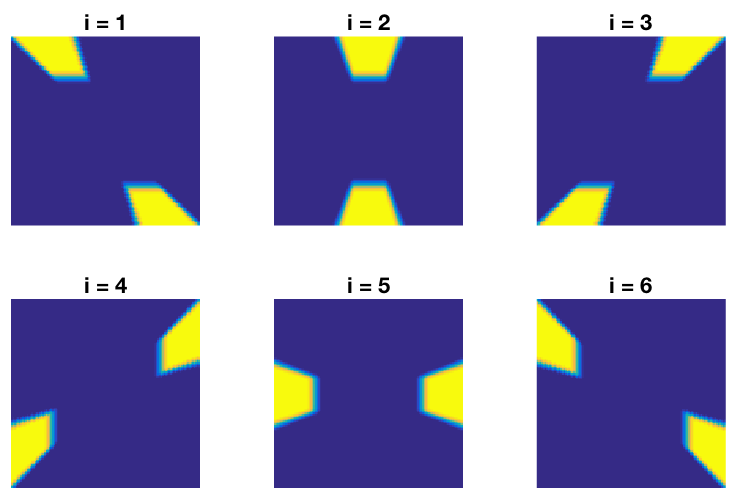
\includegraphics[width=.8\textwidth]{initialize_mdual.png}
\caption{ Input $|\m{j}|$ constructed in the same way as shearlets.}
\label{fig: mjdual}
\end{figure}

\begin{figure}
\centering
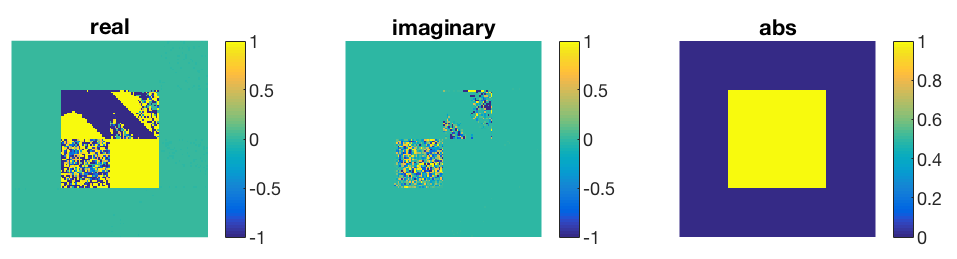
\includegraphics[width=\textwidth]{m0.png}
\caption{ $m_0(\V{\omega})$ constructed from $\widetilde{m_j}$. Left to right: $Re(m_0(\V{\omega})),\, Im(m_0(\V{\omega}))$ and $|m_0(\V{\omega})|$.}
\label{fig: m_0}
\end{figure}

\begin{figure}
\centering
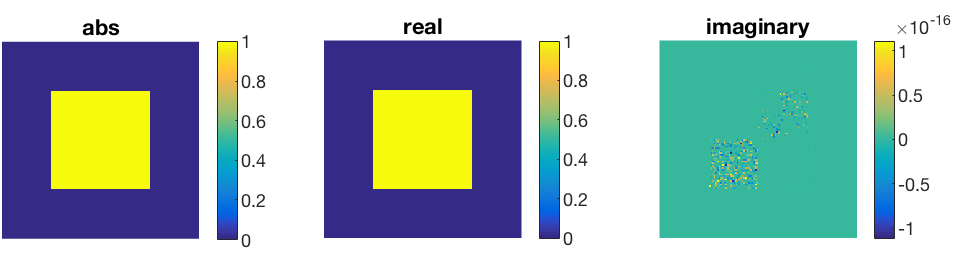
\includegraphics[width=\textwidth]{m0_m0dual_new.png}
\caption{$|\m{0}|$ and $m_0\sbarm{0}$, where $\m{0}$ is solved by optimization \eqref{eq: opt}, given $\widetilde{m_j}$ in Figure \ref{fig: mjdual} and $m_0$ in Figure \ref{fig: m_0}. Left to right: $|\m{0}|$, $Re(m_0\sbarm{0})$ and $Im(m_0\sbarm{0})$. }
\label{fig: m_0_m0dual}
\end{figure}

\begin{figure}
\centering
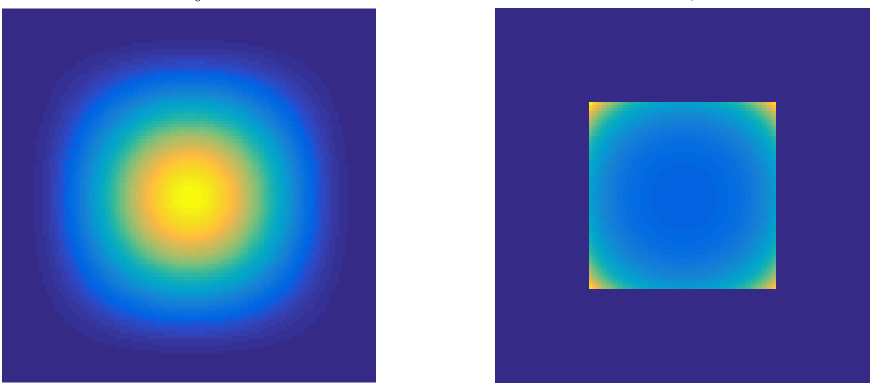
\includegraphics[width=.66\textwidth]{smooth_m0dual.png}
\caption{ Left: $\widetilde{m_0}'$, designed smooth function mainly supported on the central square $C_0$, right: $m_0'$, where $\;\, m_0'\overline{\widetilde{m_0}'}(\V{\omega})  =  m_0\sbarm{0}= \V{1}_{C_0}(\V{\omega})$. } 
\label{fig: smooth_m0dual}
\end{figure}

\begin{figure}
\centering
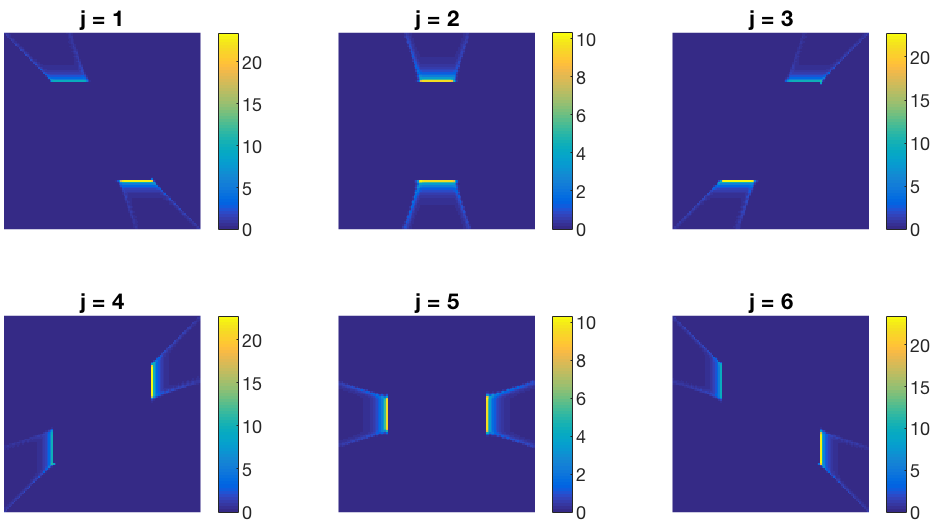
\includegraphics[width=\textwidth]{m.png}
\caption{ $|m_j(\V{\omega})|$, where $m_j(\V{\omega})$ is solved from \eqref{eq: mj-eq} given $\widetilde{m_j}$ in Figure \ref{fig: mjdual}, $m_0'$ and $\widetilde{m_0}'$ in Figure \ref{fig: smooth_m0dual}. }
\label{fig: m_j}
\end{figure}

\begin{figure}
\centering
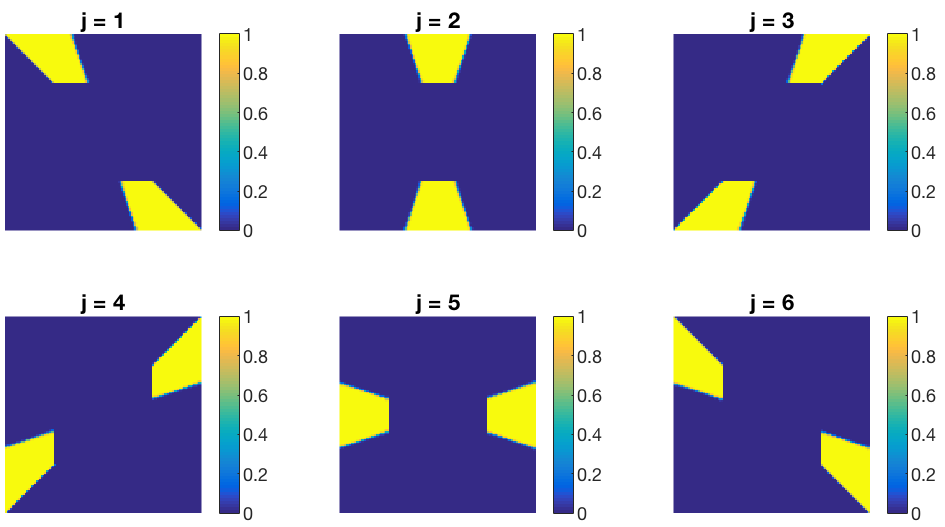
\includegraphics[width=\textwidth]{m_mdual.png}
\caption{ $|m_j(\V{\omega})\m{j}|$ for $m_j$ in Figure \ref{fig: m_j} and $\widetilde{m_j}$ in Figure \ref{fig: mjdual}. }
\label{fig: m_j_mjdual}
\end{figure}

\begin{figure}
\centering
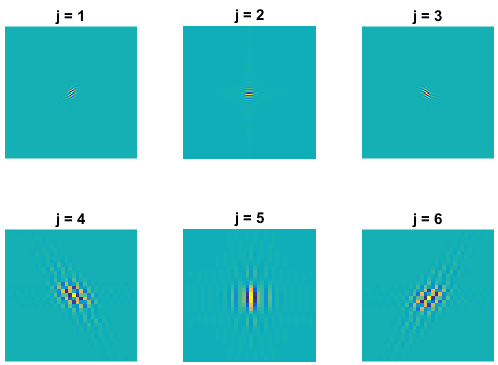
\includegraphics[width=.8\textwidth]{quincunx_wavelets.png}
\caption{ Real part of $\psi^j$ constructed from $\widetilde{m_0}'$ in Figure \ref{fig: smooth_m0dual} and $\widetilde{m_j},\, j=1,\cdots, 6$ in Figure \ref{fig: mjdual} using \eqref{eq: mj_dual}. Top: $\widetilde{\psi^j}$ without scaling, bottom: $\widetilde{\psi^j}$ with eight time zoom-in } 
\label{fig: wavelets}
\end{figure}


\begin{comment}
\subsection{solving $m_0^C$}
A set of $\m{i}$ that satisfy the conditions of Theorem \ref{thm: thm} with phase terms in \eqref{eq: phase-sol} is used as the input of \eqref{eq: LS-new}.
The left figure in Fig.\ref{fig: tm_i_m_0} shows the absolute value of $\m{i}$. In particular, $\m{i} =0,\,\forall \omega\in S_1$. 
We follow the construction process in Section \ref{subsec: compute-m0} and obtain $m_0^C$ shown in the right of Fig.\ref{fig: tm_i_m_0}, in both normal scale and log scale.  
We perform a numerical sanity check on the necessary condition in Proposition \ref{prop: feasibility}, that is $\forall\,\V{\omega}, \,s.t. [m_0(\V{\omega}), m_0(\V{\omega}+\V{\pi}_2),m_0(\V{\omega}+\V{\pi}_4),m_0(\V{\omega}+\V{\pi}_6)]$ is not a linear combination of the rows of $\mathfrak{D}(\V{\omega})$ in \eqref{eq: singular-cond}. Equivalently, we compute the following quantity $$\vartheta = 1 - \Vert V^\top\mathfrak{m}_0 \Vert/\Vert \mathfrak{m}_0\Vert ,$$ where $\mathfrak{m}_0(\V{\omega})=[m_0(\V{\omega}), m_0(\V{\omega}+\V{\pi}_2),m_0(\V{\omega}+\V{\pi}_4),m_0(\V{\omega}+\V{\pi}_6)]^\top$ and $V$ are the left singular vectors of $\mathfrak{D}(\omega)$ whose corresponding singular values are non-zero. If $\mathfrak{m}_0\in span(V)$, then $\vartheta = 0$. If $\mathfrak{m}_0\bot span(V)$, then $\vartheta = 1$.
Fig.\ref{fig: feasible} shows the feasibility check $\vartheta$ of input $\m{i}$, and $\mathfrak{m}_0$ is orthogonal to $span(V)$ everywhere.

\begin{figure}
\centering
\begin{minipage}[c]{.48\textwidth}
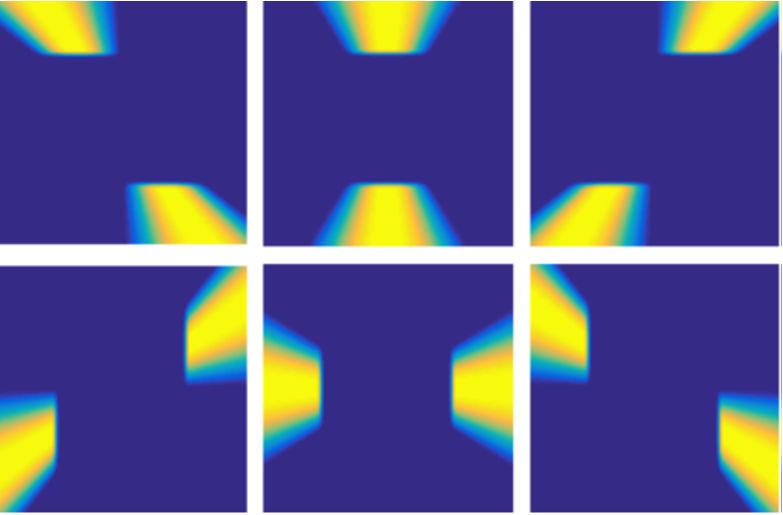
\includegraphics[width=\textwidth]{feasible_mi.pdf}
\end{minipage}
\begin{minipage}[c]{.22\textwidth}
\centering
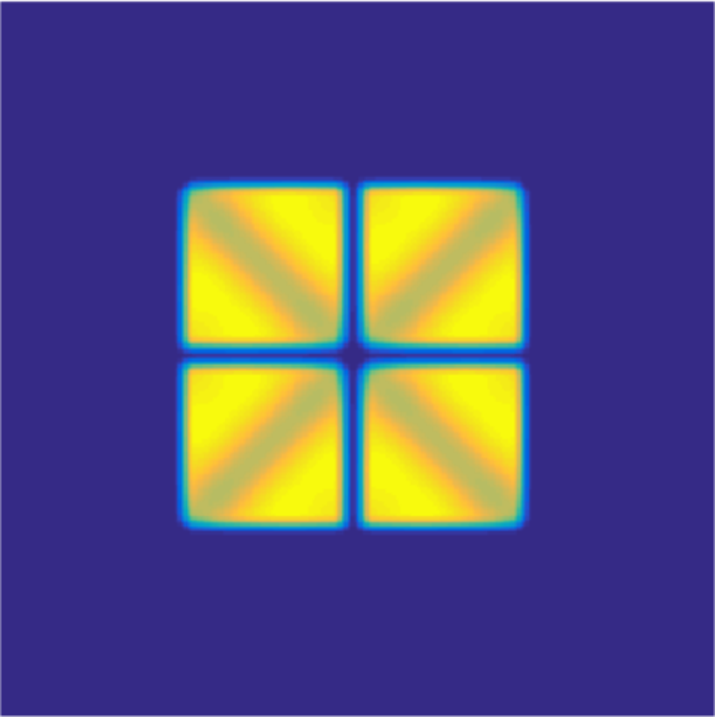
\includegraphics[width=.8\textwidth]{feasible_m0.pdf}
\end{minipage}
\begin{minipage}[c]{.28\textwidth}
\centering
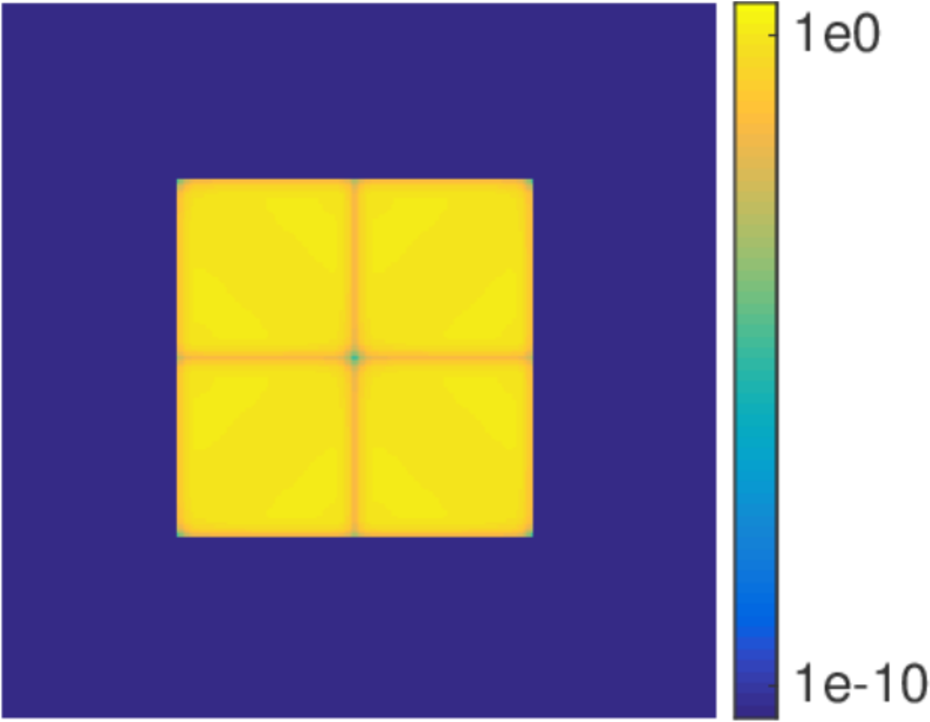
\includegraphics[width=.8\textwidth]{feasible_m0_log.pdf}
\end{minipage}
\caption{Left:  $|\m{i}|$, middle: computed $m_0^C$, right: $\log(m_0^C)$}
\label{fig: tm_i_m_0}
\end{figure}

\subsection{solving $\mc{0}$ and $m_i$}
We compute $\mc{0}$ by solving the following optimization problem similar to \eqref{eq: opt-diff} for the dyadic scheme,
\begin{align}
\min_{\xvec}\; \Vert \V{D}(\mathbf{m}_0^C\circ\xvec)\Vert^2 + \lambda\Vert \wvec\circ\mathbf{m}_0^C\circ\xvec\Vert^2,\quad 
s.t. \; A\xvec = \mathbf{1},\, \mathfrak{D}\xvec = \mathbf{0}
\label{eq: opt-2d}
\end{align}
where $\circ$ is Hadamard product and $\wvec$ is a weight vector and we consider real solution $\xvec$ here.
$A$ in the constraint is the matrix generated from the identity condition \eqref{eq: identity-cond} and $\mathfrak{D}$ is generated from the singularity condition \eqref{eq: singular-cond}. Since $A$ and $\mathfrak{D}$ are linearly independent, \eqref{eq: opt-2d} is feasible. Here, instead of optimizing the properties of $\xvec$ as in \eqref{eq: opt-diff}, we optimize those of $\widetilde{\mathbf{m}_0}^C\circ \xvec$ since $m_0^C \cdot\widetilde{m_0}^C$ will be later re-decomposed into $m_0$ and $\widetilde{m_0}$. In addition, if $m_0^C$ is symmetric with respect to the two coordinates $\omega_x$ and $\omega_y$, then we impose the same symmetry on $\widetilde{m_0}^C$ by solving \eqref{eq: opt-2d} on $[0,\pi)\times[0,\pi)$ and then extend the solution to $[-\pi,\pi)\times[-\pi,\pi)$ by symmetry.

\begin{figure}
\centering
\begin{minipage}[c]{.3\textwidth}
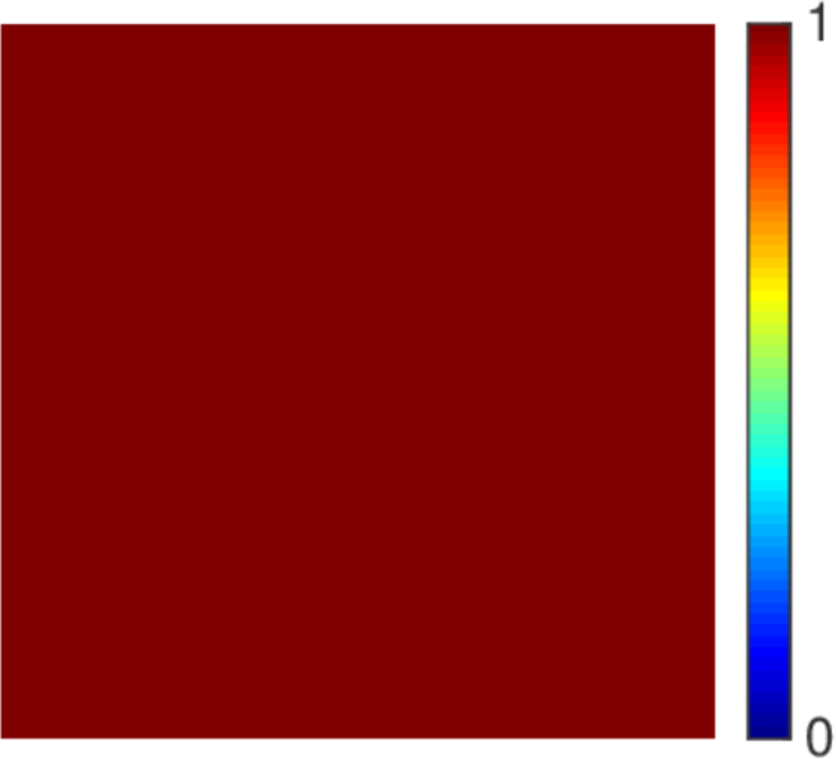
\includegraphics[width = .8\textwidth]{feasible_check.pdf}
\caption{$\vartheta$}\label{fig: feasible}
\end{minipage}
\begin{minipage}[c]{.63\textwidth}%{.28\textwidth}
\centering
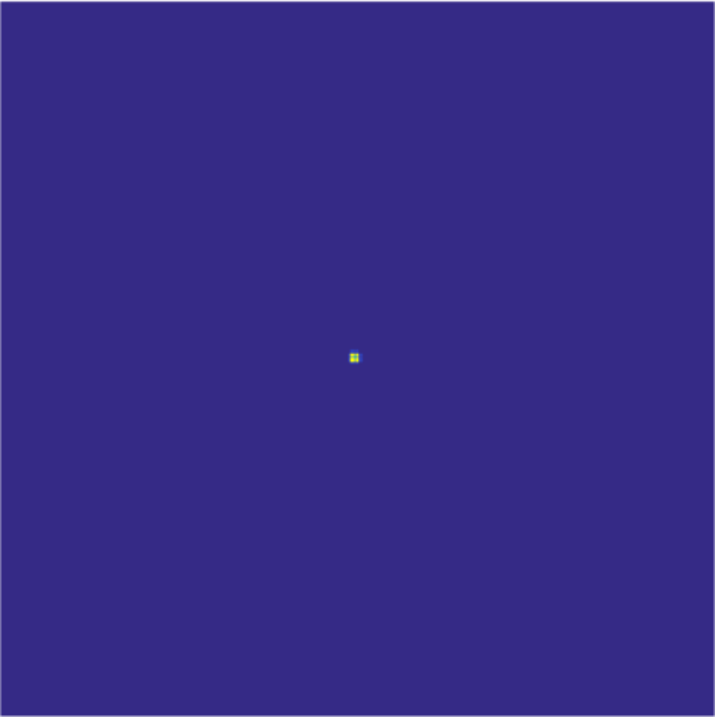
\includegraphics[width = .38\textwidth]{feasible_tm0.pdf}\hspace*{2em}
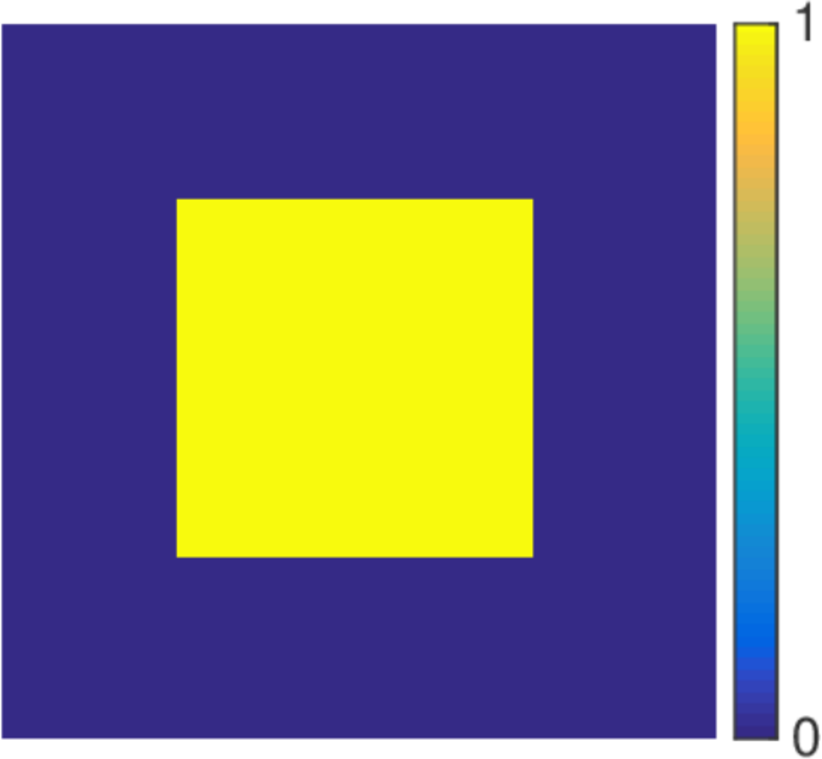
\includegraphics[width = .42\textwidth]{feasible_m0tm0.pdf}
\caption{Left: : computed $\widetilde{m_0}^C$, right: $\widetilde{m_0}^C \cdot m_0^C $}
\label{fig: tm0}
\end{minipage}
\end{figure}

Fig.\ref{fig: tm0} shows $\mc{0}$ obtained from \eqref{eq: opt-2d} and $\widetilde{m_0}^C \cdot m_0^C$ which is $\mathbf{1}_{S_1}$.

In particular, given $\widetilde{m_0}^C \cdot m_0^C = 1$, $\mathbf{b}(\V{\omega}) = \mathbf{0}, \, \forall\,\V{\omega}\in S_1$, hence $\mathbf{m}[2:7] = \mathbf{0}$. 
When $\mathbf{b}(\V{\omega})\neq \mathbf{0}$, \eqref{eq: mi} is a degenerated over-determinant linear system (we also do a sanity check here for the linearity between $\overline{\M}[:,2:7]$ and $\mathbf{b}$ by computing $\vartheta$) and 
$$\mathbf{m}[2:7](\V{\omega}) = \Big(\overline{\M}[:,2:7]\Big)^\dagger\,\mathbf{b}(\V{\omega}),$$
where $\dagger$ is the pseudo-inverse of a matrix. Fig.\ref{fig: m_i} shows the solution $m_i$ of \eqref{eq: mi} and the corresponding spatial filters $\mathcal{F}^{-1}\widetilde{m_0}$.
As shown in Fig.\ref{fig: m_i}, the energy of $m_i$ concentrates on $\{|\omega_x| = \frac{\pi}{2},\, |\omega_y| = \frac{\pi}{2}\}$ where $|\widetilde{m_i}|$ is small, and the filters decay slowly in time domain.

The bi-orthogonal bases constructed is not ideal, despite the regularization on $m_0$ in the optimization \eqref{eq: opt-2d}. Since no explicit regularization is put on $m_i$, it's difficult to control the regularity of the output $m_i$ from the input $\widetilde{m_i}$.

\begin{figure}
\centering
\begin{minipage}[c]{.5\textwidth}
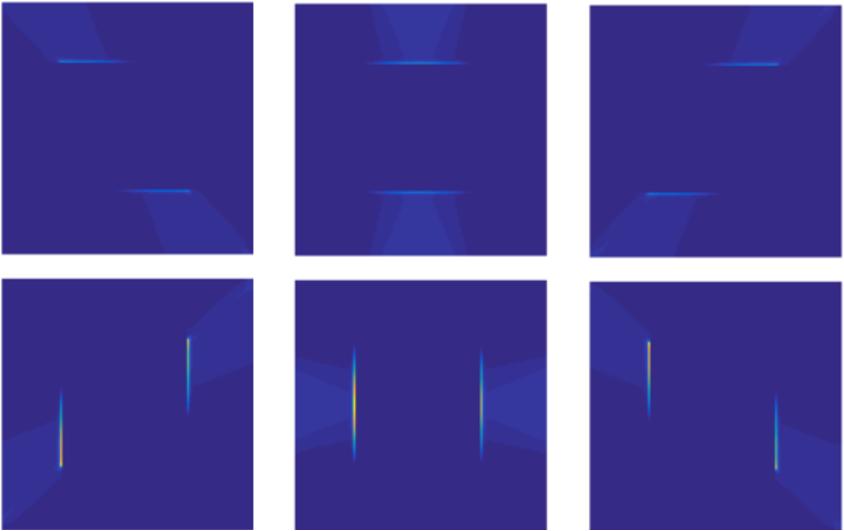
\includegraphics[width = .9\textwidth]{feasible_m.pdf}
\end{minipage}
\begin{minipage}[c]{.48\textwidth}
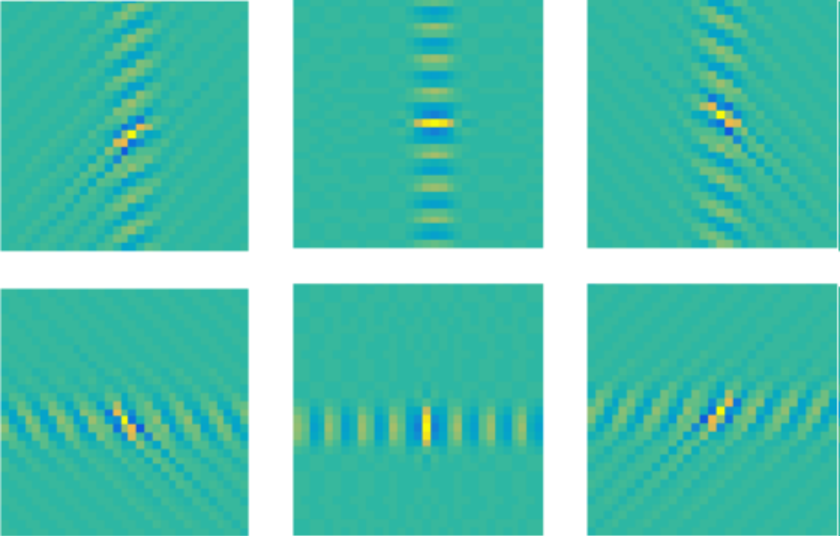
\includegraphics[width = .9\textwidth]{feasible_mi_time.pdf}
\end{minipage}
\caption{Left: $|m_i|,\, i = 1,\cdots,6$, right:$|\mathcal{F}^{-1}m_i|$}
\label{fig: m_i}
\end{figure}
\end{comment}